%%% Time-stamp: <mainrep.tex 19:57, 17 Jul 2016 by P Sunthar>
%%% $Log:$
% This document describes how to use iitbreport style
%********************************************************************

%\documentclass[11pt,a4paper,openright]{report}
\documentclass[twoside]{iitbreport}

%% Default spacing: 1.5
%% Default font size: 12pt
%% Default font: txfonts (similar to times new roman) 

%% Selectively comment out sections that you want to be left out but
%% maintaining the page numbers and other \ref
% \includeonly{%
%   intro/introduction,
%   lit/literature,
%   expt/experimental,
%   rnd/results, 
%   dec,abs,pub,ack
% }

%%% Some commonly used packages (make sure your LaTeX installation
%%% contains these packages, if not ask your senior to help installing
%%% the packages)

\setlength {\marginparwidth }{2cm}
\usepackage{todonotes}

\usepackage{booktabs}
\usepackage{array}
\usepackage{tabularx}
\renewcommand\tabularxcolumn[1]{m{#1}}
\usepackage[export]{adjustbox}

%%% Macro definitions for Commonly used symbols
\newcommand{\Rey}{\ensuremath{\mathrm{Re}}}
\newcommand{\avg}[1]{\ensuremath{\overline{#1}}}
\newcommand{\tenpow}[1]{\ensuremath{\times 10^{#1}}}
\newcommand{\pder}[2]{\ensuremath{\frac{\partial#1}{\partial#2}}}

% Referencing macros
\newcommand{\Eqref}[1]{Equation~\eqref{#1}}
\newcommand{\Tabref}[1]{Table~\ref{#1}}
\newcommand{\Figref}[1]{Figure~\ref{#1}}
\newcommand{\Appref}[1]{Appendix~\ref{#1}}


\begin{document}
	
%%********************************Frontmatter***********************
% In frontmatter everything comes with roman numbering	
\pagenumbering{roman}
\setcounter{page}{1}

%*******************************************************************
%                         Title Page                            
%*******************************************************************
\title{Feature Preserving Face Redaction of Videos in Indoor Settings}
\author{Abhinav Kumar}

%% Print the date. Today's date comes by default, change it here to 
%% other date format, if required:

%\date{\today}
% \date{23 June, 2022}


%% The type of the report can be set here

\reporttype{MTech Project Report}
% \reporttype{A Seminar Report}
%\reporttype{A Thesis}
%\reporttype{A Dissertation}
%\reporttype{A Project Report}

%% Name of the degree
% \degree{Doctor of Philosophy}
\degree{Master of Technology}


%% Department/Centre Name
\dept{Department of Computer Science \& Engineering}

%% Supervisor and cosupervisor/excosupervisor are not essential parts
%% of a report title page, as it is your report!

%% But if you **have** to put it uncomment these
\supervisor{Prof. Sharat Chandran}
%\cosupervisor{Co-super name}
%\excosupervisor{External Supervisor}

%% Roll number
\rollnum{19305R001}

\maketitle

%*******************************************************************
%                         Copyright Page                          
%******************************************************************* 
%\mycopyright                    

%*******************************************************************
%                         Dedication Page                         
%*******************************************************************
\dedication[Dedicated to \ldots \\ my mother, Mrs. Manju Singh \\ and \\ my father, Mr. Dharmendra Kumar Singh]
%\addintoc{Dedication}

%*******************************************************************
%                        Certificate Page                         
%*******************************************************************
%\makecertificate[change title name]{report type} 
% \makecertificate{seminar report} 
%\makecertificate{thesis}
%\makecertificate{dissertation}
\makecertificate{MTech Project report}

%\addintoc{Certificate}

%*******************************************************************
%                         Approval Sheet                         
%*******************************************************************
\makeapproval{MTech Project report}
% \makeapproval{dissertation}

%*******************************************************************
%                          Declaration                           
%*******************************************************************
%==================================dec.tex================================
%
\begin{Declaration}
\noindent
I declare that this written submission represents my ideas in my own words and where others' ideas or words have been included, I have adequately cited and referenced the original sources. I declare that I have properly and accurately acknowledged all sources used in the production of this report. I also declare that I have adhered to all principles of academic honesty and integrity and have not misrepresented or fabricated or falsified any idea/data/fact/source in my submission. I understand that any violation of the above will be a cause for disciplinary action by the Institute and can also evoke penal action from the sources which have thus not been properly cited or from whom proper permission has not been taken when needed.

%
%
%
%
%
%
%

\DecSign[\today]


%
\end{Declaration}
%========================================================================
















 
%\addintoc{Declaration}

%******************************************************************
%                          Abstract                             
%******************************************************************  
%============================= abs.tex================================
\begin{Abstract}
Analysis of mental health and development from videos is a relatively newer field in scene understanding from computer vision algorithms. A vital feature utilized for such behavioral analyses is the gaze of the subject. For instance, the so-called Preferential Looking and the Anti-saccade tasks adopted in the Autism community track the gaze for 2-Way and 3-Way Gaze Classification, respectively. Another important feature for gauging the subject's attention is the proximity of the face to the camera of the recording device. To this end, we prepare a Gaze Tracking dataset to facilitate mental health assessments.\\

It is imperative to preserve the identities of the subjects before releasing the dataset, which leads to Face Redaction. It is the task of hiding all the faces present in the dataset. There are several ways in which the faces can be redacted, e.g., by blurring or blackening out all the faces, swapping the face with the face of another person, or overlaying a mesh of facial landmarks. In this work, we achieve face redaction by blurring or blackening out the faces. Face redaction makes it difficult to extract gaze and facial features from redacted faces. In this work, we propose a \textbf{Feature Preserving Redaction} mechanism that preserves the important features required for further analyses. Many applications demand such a feature preserving nature of redaction, e.g., releasing a dataset while preserving the privacy of the subjects, hiding the identity of a public figure or students appearing in a remote exam before analyzing the scene, etc. Since these videos are recorded in an unproctored environment, we systematically demonstrate the versatility of our methods in an uncurated setting via several experiments.


%
%
%
%
%
\end{Abstract}
%=======================================================================

                    

%******************************************************************
%                         Contents list                         
%******************************************************************
%\figurespagefalse
%\tablespagefalse
\makecontents % Creats toc, lof, and lot

%******************************************************************
%                        Notations                              
%******************************************************************
%\notations[4cm]{List of Symbols}
%\todo{Remove List of Symbols if not used. Possible usage: ASD}

%%********************************Mainmatter***********************
% In mainmatter everything comes with arabic numbering	
\cleardoublepage
\setcounter{page}{1}
\pagenumbering{arabic}

%******************************************************************
%                         Chapters                           
%****************************************************************** 
\chapter{Introduction}

% Justify & highlight the problem
Behavioral analysis and the analysis of mental health and development from videos utilizing computer vision algorithms is a relatively newer field adopted in the Autism community. Most works done till date try to interpret and identify the objects present in the scene and extract physical and geometrical parameters like pose, orientation, location, etc. Along similar lines, the gaze of a subject and the proximity of the subject’s face from the recording device are some of the important features utilized for gauging the social and non-social preferences of the subject in the Autism community and carrying out various mental health assessments.

In this direction, we prepare a Gaze Tracking dataset containing videos of children aged 0-6 years performing Preferential Looking Task on a tablet in indoor settings. This dataset is targeted toward the screening and classification of Autism Spectrum Disorder (ASD) in small children and will be helpful for the Autism community. Before releasing the dataset to the community, the primary concern is the redaction of the identities of the subjects present in the video (since our dataset is subject to GDPR regulations). So, our aim is to share a face redacted dataset while preserving the gaze and facial proximity features of the subjects. In this work, we aim to systematically demonstrate our feature preserving approach to face redaction using the ITracker neural network as the base model introduced by \cite{MIT_EyeTracking_paper} and prepare a feature-rich face redacted dataset.


%%%%%%%%%%
\section{Face Redaction}
Redaction refers to the process of hiding some sensitive information present in an image in order to preserve the privacy of individuals. The sensitive information can be present in the foreground or the background of the image. An example of the redaction of the foreground is the face redaction problem, which aims at preserving the identities of the subjects present in the videos. There are several ways in which the faces can be redacted, e.g., by blurring or blackening out all the faces, swapping the face with the face of another person, or overlaying a mesh of facial landmarks. For the sake of simplicity, we blur or blacken out the faces present in the video. The various modalities in which face redaction can be achieved are demonstrated in figure \ref{fig:faceRedactModes}. The face can either be blurred or completely blacked out to hide the identity, or the facial landmarks can be overlaid on the black background or the blurred face. As we will demonstrate the importance of eyes for gaze tracking in upcoming sections, the eyes can either be hidden or visible in each of the above modalities.

\begin{figure}[tbp]
  \centering
    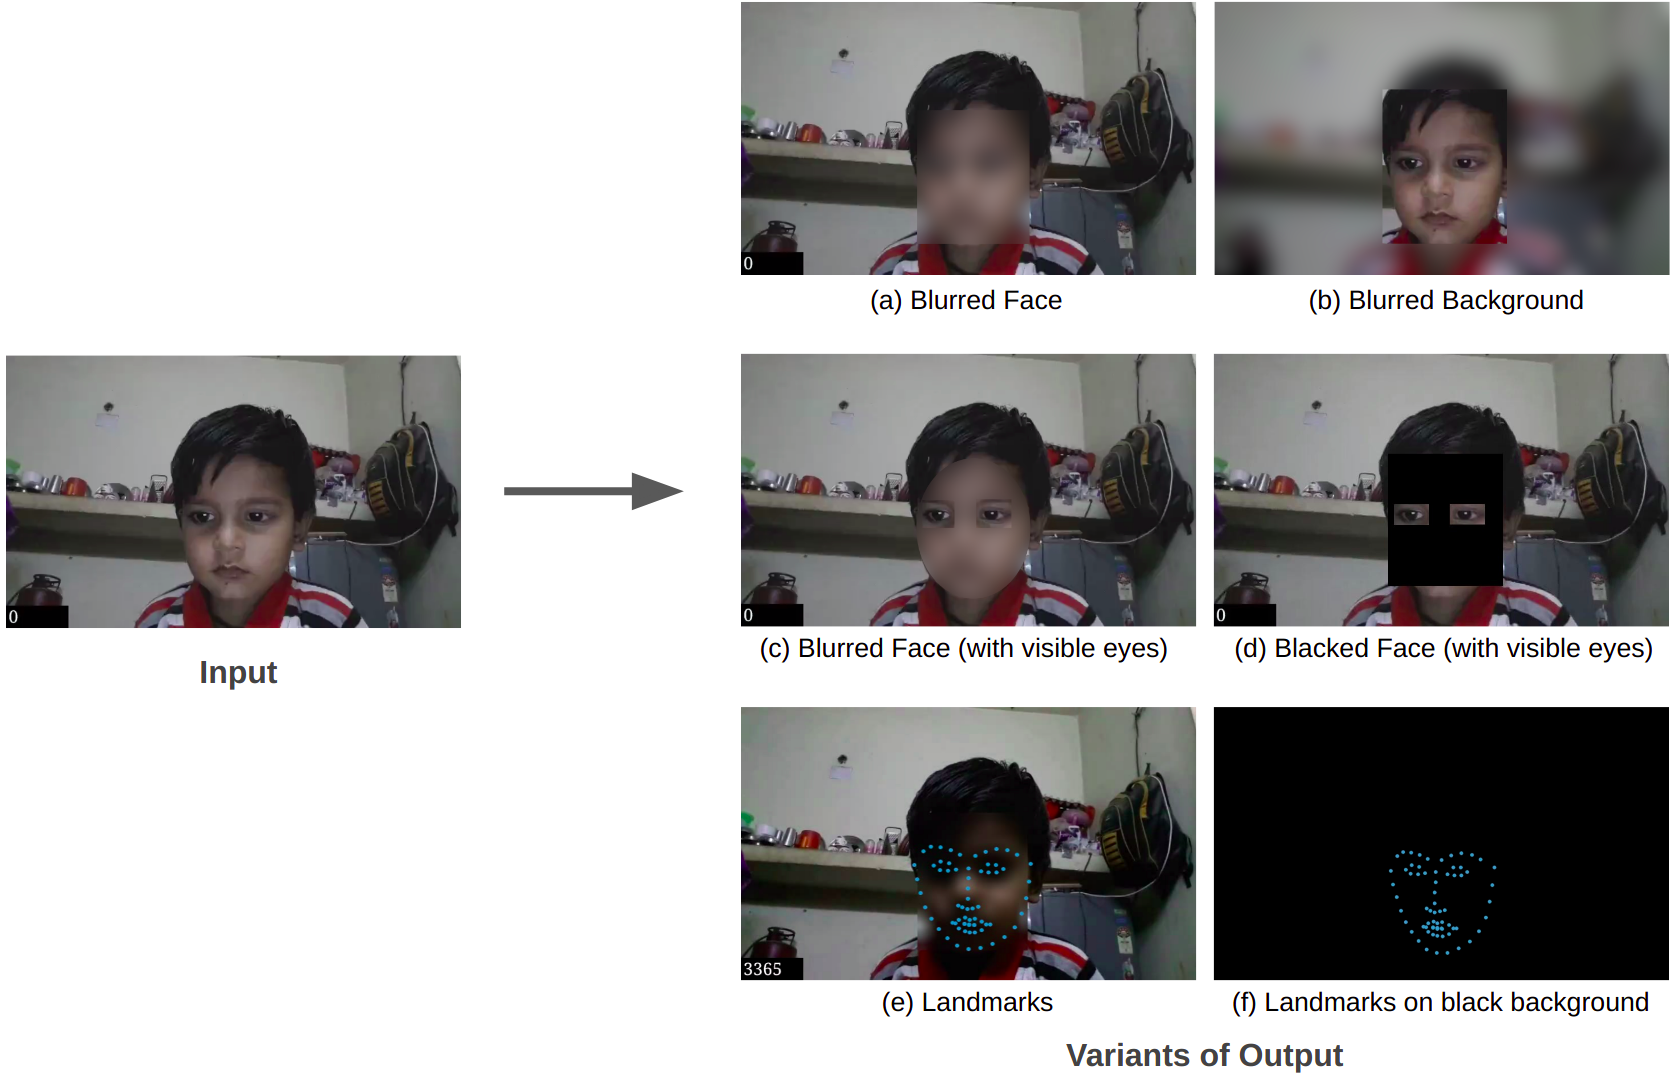
\includegraphics[width=1.0\textwidth]{Introduction/FaceRedactionModalities}
    \caption[Redaction Modalities]{Redaction modalities}
    \label{fig:faceRedactModes} 
\end{figure}

While this procedure is of utmost importance before releasing the dataset to the community, it makes it difficult to extract gaze and facial proximity features from these redacted faces. Thus, a feature preserving redaction mechanism needs to be adopted.


%%%%%%%%%%
\section{Gaze Classification}
Gaze refers to the direction in which an individual is looking and focusing at. This is an important feature of an individual's behavioral aspect which makes the tracking of an individual's gaze very vital in order to study the attention of the individual. The task of Gaze Tracking (or sometimes Eye Tracking) refers to the use of an external device to follow an individual’s gaze and eye movement, which is used for various studies, including studies of the visual system, cognition, and psychology. In such applications, one is typically interested in the classification of gaze into Left or Right regions (called 2-Way Classification, figure \ref{fig:2wayGazeClassif}) or Left, Right, or Middle regions (called 3-Way Classification, figure \ref{fig:3wayGazeClassif}) of the device on which the eye-tracking data is collected. An application running on a device (say, a mobile phone) displays a dot (fixation point), the subject looks at the fixation point, video of the subject is recorded using the front camera of the device, which is used to monitor the screen location where the subject is looking at.\\

\begin{figure}[h]
    \centering
    \captionsetup[subfigure]{justification=centering}
    \subfloat[2-Way Gaze Classification on Preferential Looking Task]{{
        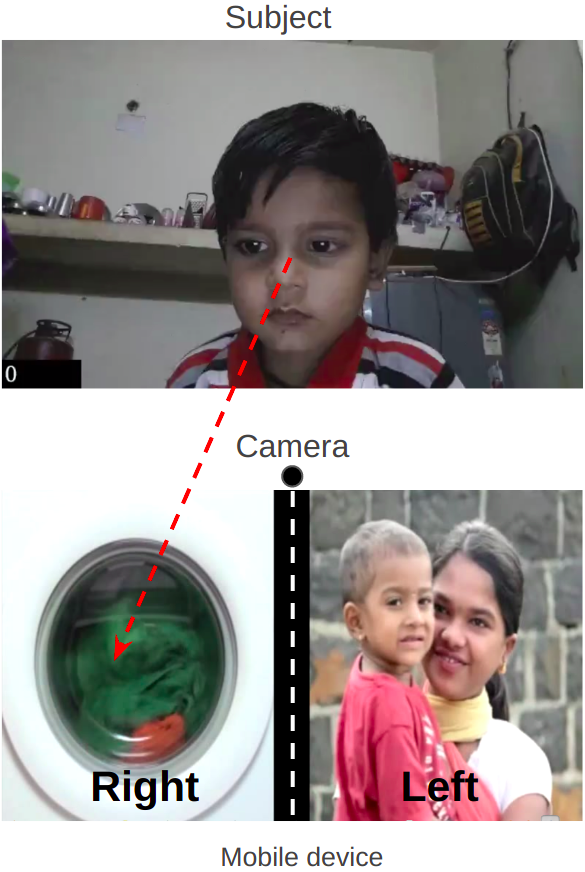
\includegraphics[scale=0.3]{Introduction/2wayGazeClassif}
        \label{fig:2wayGazeClassif}
        }}
    \qquad
    \subfloat[3-Way Gaze Classification on Anti-Saccade Task]{{
        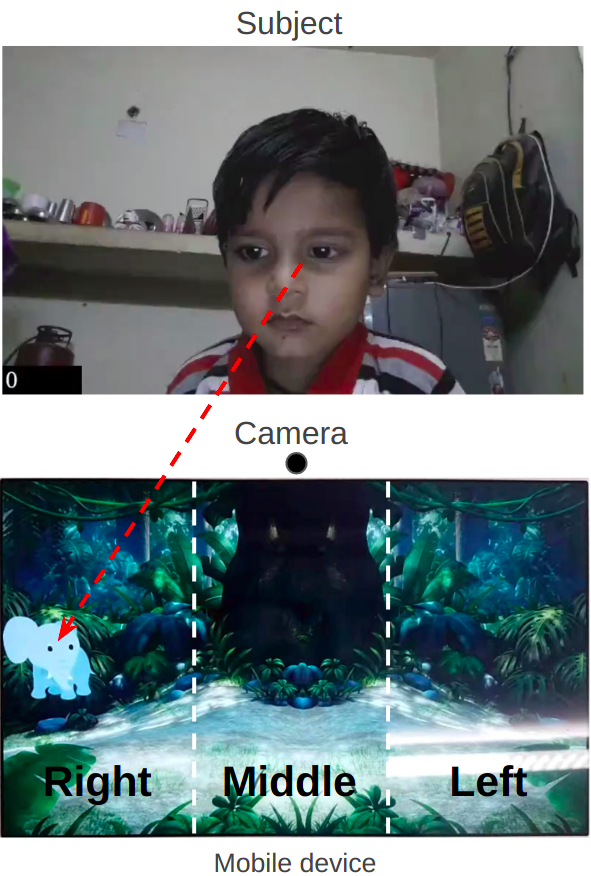
\includegraphics[scale=0.3]{Introduction/3wayGazeClassif}
        \label{fig:3wayGazeClassif}
    }}
    \caption{Gaze Classification}
\end{figure}


%%%%%%%%%%
\section{Facial Proximity}
The proximity of the face to the camera of the recording device is an important feature for gauging the attention of the subject. We extract the 3-D facial landmarks using the state-of-the-art facial landmark detector, RetinaFace \citep{retinaFace2020} and calculate the relative 3-D proximity of the nose-tip from the camera across consecutive frames of the video.

\begin{figure}[h]
  \centering
    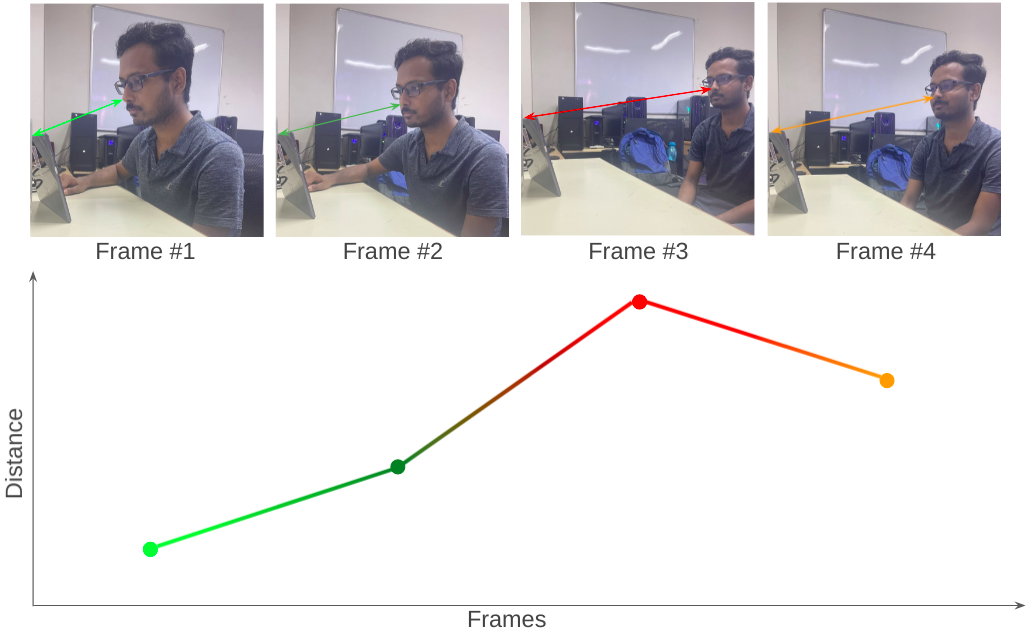
\includegraphics[width=0.85\textwidth]{Introduction/RelFaceDist}
    \caption[Relative Face Proximity]{Relative 3-D proximity of nose-tip from camera across consecutive frames}
    \label{fig:relFaceDist} 
\end{figure}


%%%%%%%%%%
\section{Motivation and Applications}
We need to share our prior work and results obtained on our Gaze Tracking dataset. Given that our Gaze Tracking Dataset is subject to GDPR regulations, identity preservation is imperative, without which we can’t share the dataset. Therefore, we aim to prepare and share a redacted dataset with eye crops and facial landmark coordinates in order to establish the utility of our redacted dataset for gaze classification and facial proximity calculation. With redacted faces and eye crops present in our dataset, we can calculate the gaze of an individual. The landmarks supplied along with our dataset can be used to compute the facial proximity of individuals. Our dataset can also be used for the exploration of new algorithms on a redacted dataset for research purposes.

This work finds applications in many domains. For example, gaze tracking in remote exam settings is important for tracking whether the student is looking at the screen. Malpractice detection without revealing a student’s identity in such remote exam settings is very helpful for academia. Another important metric is face distance and proximity, which is very helpful in gauging the attention of an individual. Such a pipeline can be incorporated into software applications such as SafeEyes (a Linux-based software for the protection of eyes from excessive screen exposure) without breaching the privacy of the user.

\section{Contributions}
As discussed in previous sections, the task of face redaction makes the image lose the important facial features which are required for gaze classification and proximity calculation. We propose a feature preserving face redaction pipeline, which is useful for sharing a privacy preserved dataset to the research community. Furthermore, we demonstrate the utility of such a face redacted dataset by performing several experiments and ablation studies for gaze classification on this dataset. We show that our approach to gaze classification works equally well on face redacted data as it performs on the unredacted data. Specifically, we achieve a 3-way gaze classification accuracy of 82\% and a 2-way gaze classification accuracy of 96\% on UK dataset. We test our approach on the uncurated START data collected using Preferential Looking task and achieve a 2-way classification accuracy of 93\% with redacted faces. We also proposed an algorithm to calculate the proximity of the face of an individual from the camera and demonstrate the proximity trends on various in-the-wild videos. We plan to make the trained models and face redacted dataset (along with the facial features in terms of facial landmarks and eye crops) available to the research community for further investigations and research work.
\chapter{Literature Survey}

In this section, we present the ITracker neural network introduced by \cite{MIT_EyeTracking_paper} used as our base model. We then discuss the extractors explored to extract the face and eyes required as inputs to the network. We also compare the performance of these face detectors surveyed in this work for the purpose of redaction.


%%%%%%%%%%
\section{ITracker Neural Network}
The ITracker Neural Network proposed by \cite{MIT_EyeTracking_paper} is a deep CNN that takes the face and eye crops and a face grid as inputs and predicts the XY gaze coordinates on the screen w.r.t. the camera as output. The X-coordinate and Y-coordinate axes are oriented rightwards and upwards, respectively, with the camera located at the origin of this reference frame. We leverage this model for our purposes of classification of gaze (2-Way or 3-Way) by replacing the final XY gaze regression layer with a gaze classification layer to output the gaze class labels.

\begin{figure}[h]
  \centering
    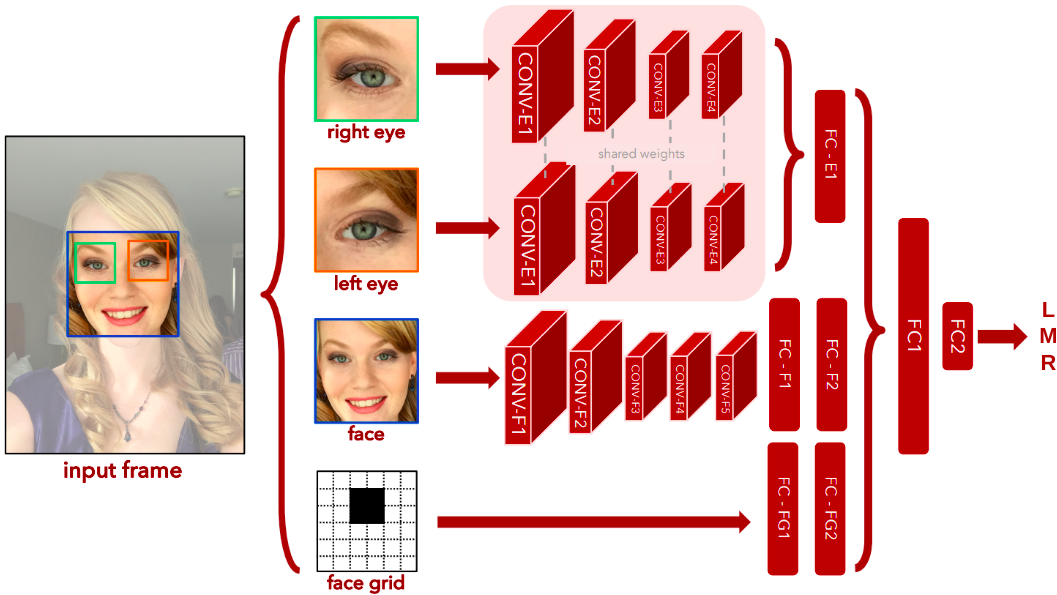
\includegraphics[width=1.0\textwidth]{LiteratureSurvey/ITrackerNN}
    \caption[ITracker NN]{ITracker NN for Gaze Classification}
    \label{fig:iTrackerNN} 
\end{figure}

The crops of the face and eyes are extracted from the frame by an extractor. In this work, we first use The Histogram of Oriented Gradients (HOG) face extractor provided in the Dlib library of OpenCV and RetinaFace detector for extracting face and eyes. As we explore other face detectors in the upcoming sections, we compare these and finally arrive at the best detector out of these detectors for extracting face and eyes. The face grid input to the neural network is a binary mask of the face in the entire frame.


%%%%%%%%%%
\section{S3FD: Single Shot Scale-invariant Face Detector}
S3FD is based on the state-of-the-art SSD object detection framework \cite{ssd2016} where, unlike the detection and classification module, which occurs at the end of the architecture pipeline in a Region Proposal Network, the detection and classification are performed at various levels of feature maps. As depicted in figure \ref{fig:s3fdNN}, the shallow feature map has a small receptive field, which is responsible for and drastically improves the detection of small-scale faces. On the other hand, the deep feature map has a large receptive field, which is responsible for the detection of large-scale faces. 

\begin{figure}[h]
  \centering
    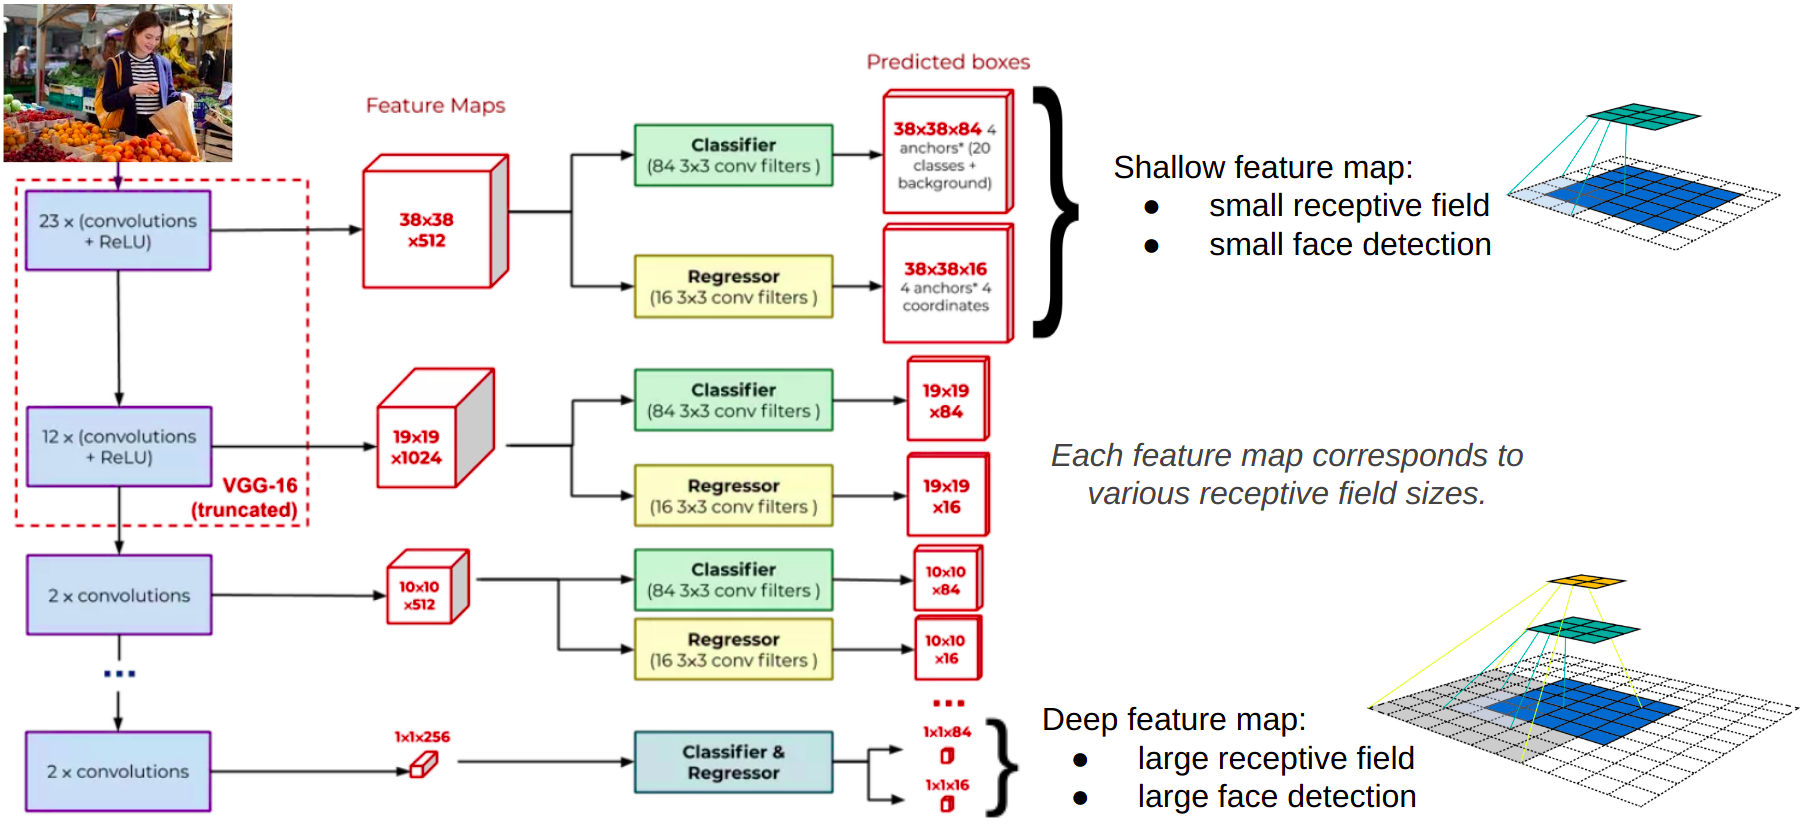
\includegraphics[width=1.0\textwidth]{LiteratureSurvey/S3FD_NN}
    \caption[S3FD]{S3FD NN Architecture}
    \label{fig:s3fdNN} 
\end{figure}

\paragraph{Designing Anchor Scale}
In addition to the scale-invariant detection framework discussed above, the anchor scales at different levels of feature maps are designed on the basis of Effective Receptive Field (ERF) at that level, as shown in figure \ref{fig:anchorScaleERF}. The reasoning is that the ERF is the region in the input image, which significantly affects the detection at a particular level. So, designing anchor scales that correspond to the ERF scale helps to improve the detection rate. 

\paragraph{Max-out Background label}
Although the framework of detection at various levels of the feature map imparts scale-invariance to the network, a problem arises due to the first detection layer, as shown in figure \ref{fig:maxOutBgLabel_problem}. Due to a large number of background labels at small-scaled anchors, the face detection task gets exposed to an extremely unbalanced binary classification task and the overall false-positive rate increases for small faces.

In order to reduce the false-positive rate for small faces, the proposed solution is to predict \emph{N} scores for the background label for each anchor in the first detection layer and then select the highest score as the confidence of the background label (figure \ref{fig:maxOutBgLabel_solution}).

\begin{figure}[h]
    \centering
    \captionsetup[subfigure]{justification=centering}
    \subfloat[Designing Anchor Scale from ERF]{{
        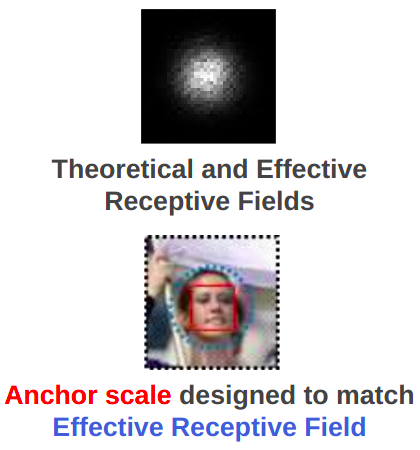
\includegraphics[scale=0.25]{LiteratureSurvey/AnchorScaleERF}
        \label{fig:anchorScaleERF}
        }}
    \quad
    \subfloat[Unbalanced Binary Classification]{{
        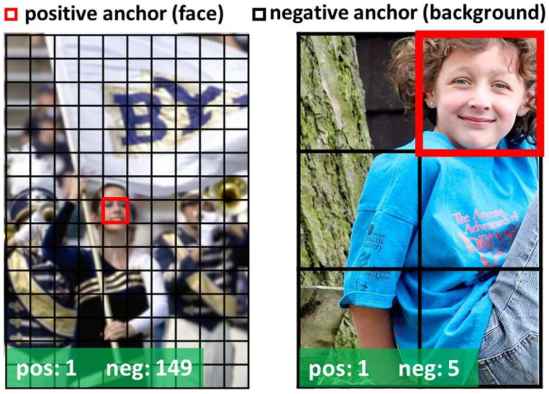
\includegraphics[scale=0.25]{LiteratureSurvey/MaxOutBgLabel_problem}
        \label{fig:maxOutBgLabel_problem}
    }}
    \quad
    \subfloat[Max-out Background Label]{{
        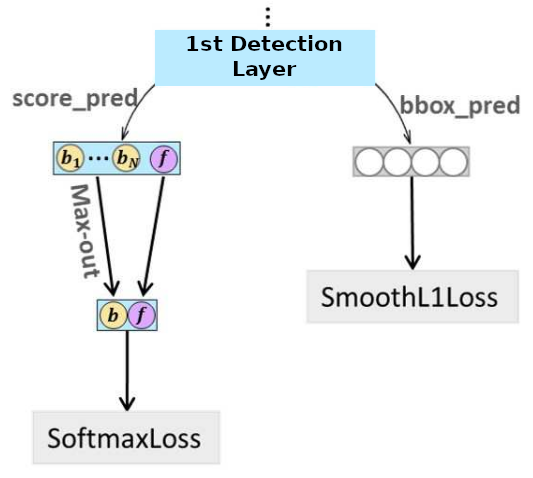
\includegraphics[scale=0.25]{LiteratureSurvey/MaxOutBgLabel_solution}
        \label{fig:maxOutBgLabel_solution}
    }}
    \caption{S3FD: Scale-invariant face detection}
\end{figure}


%%%%%%%%%%
\section{DSFD: Dual Shot Face Detector}
Dual Shot Face Detector \cite{dsfd2018} is a 2-stage detection framework that extends the idea of detection at various feature maps by introducing a Feature Enhance Module to capture a wider context for better face detection (figure \ref{fig:dsfdNN}). Similar to S3FD, it first obtains the feature maps at various levels in the Original Feature Shot. These features are then passed to Feature Enhance Module to obtain the enhanced features called Enhanced Feature Shot. Finally, a Progressive Anchor Loss (PAL) is computed from both the original and enhanced features to train the network.

\begin{figure}[h]
  \centering
    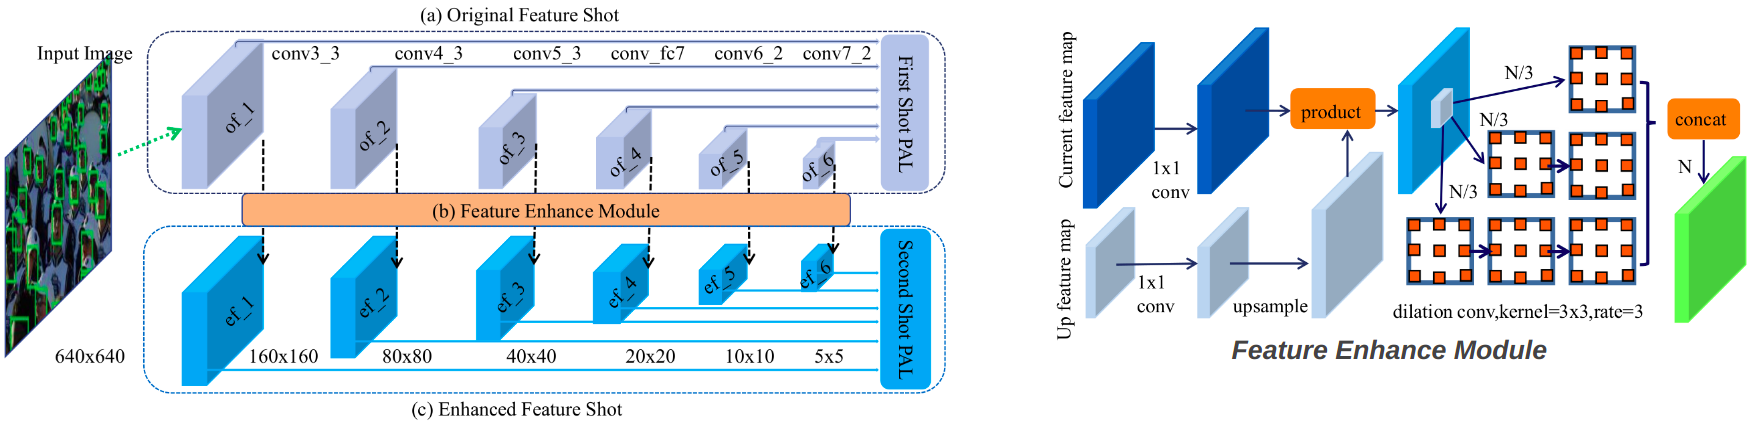
\includegraphics[width=1.0\textwidth]{LiteratureSurvey/DSFD_NN}
    \caption[DSFD]{DSFD NN Architecture}
    \label{fig:dsfdNN} 
\end{figure}

\paragraph{Feature Enhance Module}
Feature Enhance Module shown in figure \ref{fig:dsfdNN} aims to impart wider context information to the network to better detect faces, particularly at small scales. For each feature map, the feature map at the next level is upsampled and integrated with the current feature map. Since the features at the next level have a larger receptive field, this increases the context information available to the current feature map. Finally, a dilated convolution is applied on top of this integrated feature map which further helps to increase the receptive field at the current level as depicted in figure \ref{fig:dilatConvIncRF}.

\begin{figure}[h]
  \centering
    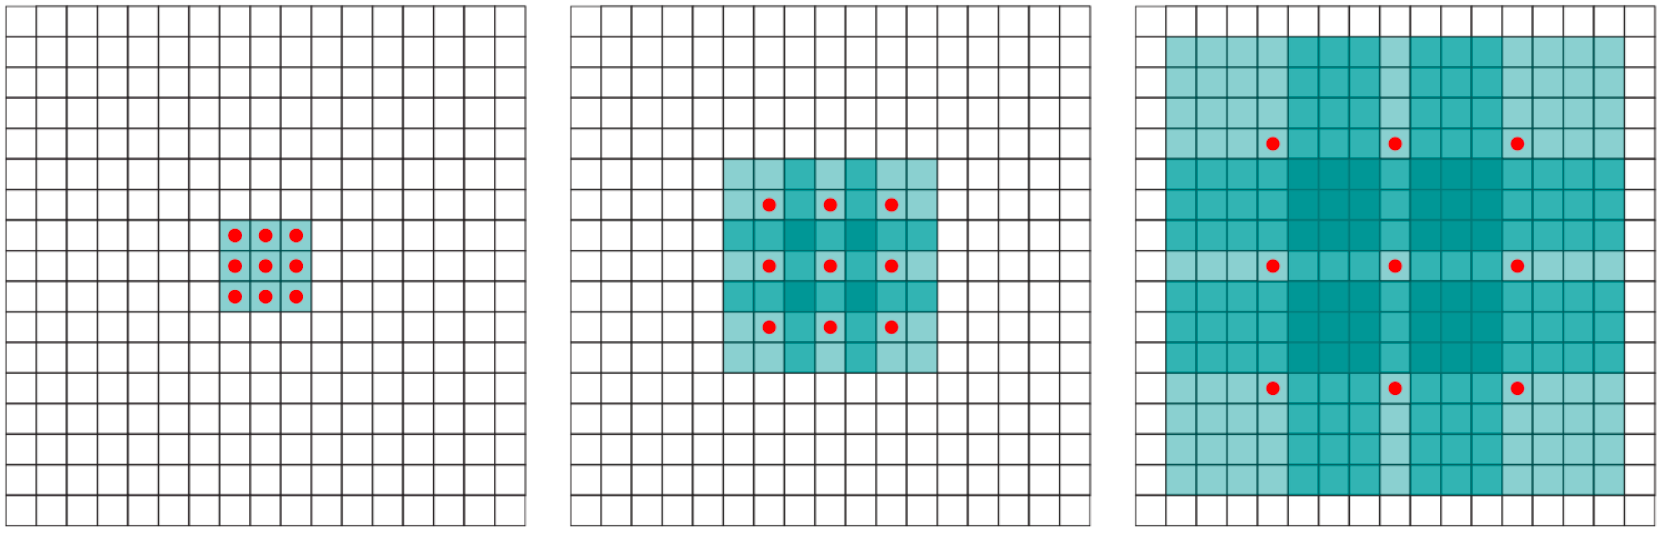
\includegraphics[width=0.7\textwidth]{LiteratureSurvey/DilatConvIncRF}
    \caption[Dilated Convolution]{Increased Receptive Field due to Dilated Convolution}
    \label{fig:dilatConvIncRF} 
\end{figure}


%%%%%%%%%%
\section{LFFD: Light and Fast Face Detector}
As the name suggests, Light and Fast Face Detector \cite{lffd2019} is designed to be a fast real-time face detector with a lightweight model for direct deployment on edge devices that have limited memory storage and low computing power. LFFD is inspired by the single-stage, and multi-scale object detection method SSD \cite{ssd2016}, which also enlightens some other face detectors. One of the characteristics of SSD is that pre-defined anchor boxes are manually designed for each detection branch. These boxes always have different sizes and aspect ratios to cover objects with different scales and shapes. Therefore, anchors play an important role in most single-stage detection methods. However, anchor-based methods may face three challenges:
\begin{enumerate}
    \item Anchor matching is unable to sufficiently cover all face scales. Although this can be relieved, it remains a problem.
    \item Matching anchors to ground-truth bounding boxes is determined by thresholding IoU. The threshold is set empirically, and it is difficult to make a solid investigation of its impact.
    \item Setting the number of anchors for different scales depends on experiences, which may induce sample imbalance and redundant computation.
\end{enumerate}

\paragraph{Anchor-free method}
The key idea is that the Receptive Field (RF) serves as a natural anchor at each detection layer. RF can easily handle the above challenges. Firstly, continuous scales of faces can be predicted within a certain RF size rather than discrete scales in anchor-based methods. Secondly, the matching strategy is clear; namely, an RF is matched to a ground-truth bounding box if and only if its center falls in the ground-truth bounding box. Thirdly, the number of RFs is naturally fixed, and they are regularly distributed in the input image.

Using RFs as anchors naturally raises the concern that faces of different sizes need different RF strategies: for tiny or small faces, Effective Receptive Field (ERF) should cover faces as well as sufficient context information, whereas for large faces, keeping faces in RF is enough, as depicted in figure \ref{fig:RFasAnchor}.

\begin{figure}[h]
  \centering
    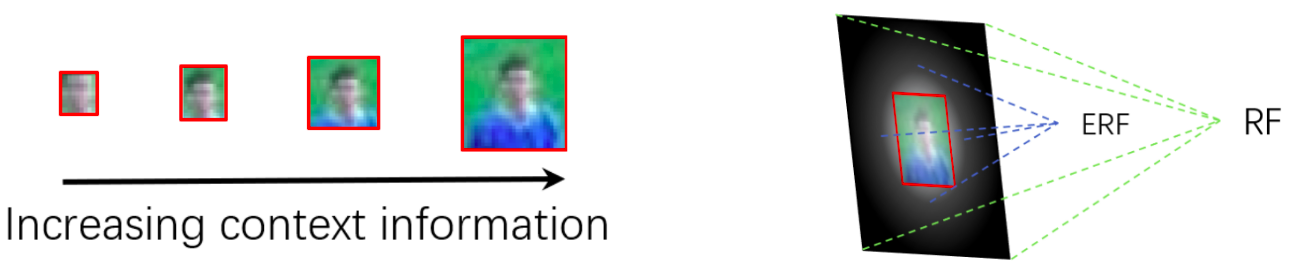
\includegraphics[width=1.0\textwidth]{LiteratureSurvey/RFasAnchor}
    \caption[Receptive Field as Anchor]{Receptive Fields as natural Anchors}
    \label{fig:RFasAnchor} 
\end{figure}


%%%%%%%%%%
\section{YOLOv5 Face}
The YOLO-based object detectors are excellent in real-time detection at high accuracy, which are utilized in many works. YOLOv5 Face Detector \cite{yolov5face2021} is based on the YOLOv5 object detector, with the redesign of some components targeted for face detection. A landmark regression module is added in the object prediction head, lightweight ShuffleNetV2 architecture is used as the backbone to reduce computations, kernel size and stride are modified for some network blocks, and data augmentation methods are optimized, specifically suited for face detection.

There is a portfolio of three YOLOv5 Face detection models available for a variety of trade-offs between speed and accuracy: small, medium, and large. Since the focus of our work is to obtain the best face detector on our dataset instead of real-time application, we run the medium and large models on our dataset.


%%%%%%%%%%
\section{Retina Face}
The key idea of the Retina Face detector \cite{retinaFace2020} is similar to YOLOv5 Face detector, i.e., incorporation of facial landmark regression with the face detection module. But Retina Face takes this idea a step further, and the network is trained for three tasks simultaneously: face bounding box, 2D facial landmarks, and 3D mesh vertices. The method uses ground-truth 3D mesh vertices (figure \ref{fig:RF_mesh}) for multi-task learning. This is a very powerful reinforcement technique since the underlying target for all tasks above is the same: accurate point prediction on the image plane, therefore each task benefits from other tasks, as shown in figure \ref{fig:RF_multiTaskBenefit}

\begin{figure}[h]
    \centering
    \captionsetup[subfigure]{justification=centering}
    \subfloat[Mesh68 and Mesh1k]{{
        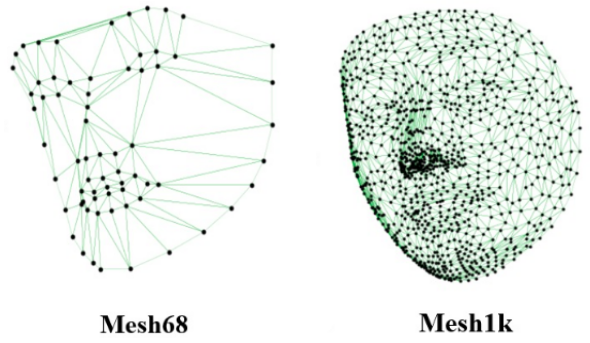
\includegraphics[scale=0.25]{LiteratureSurvey/RF_mesh}
        \label{fig:RF_mesh}
        }}
    \quad
    \subfloat[Multi-task benefit]{{
        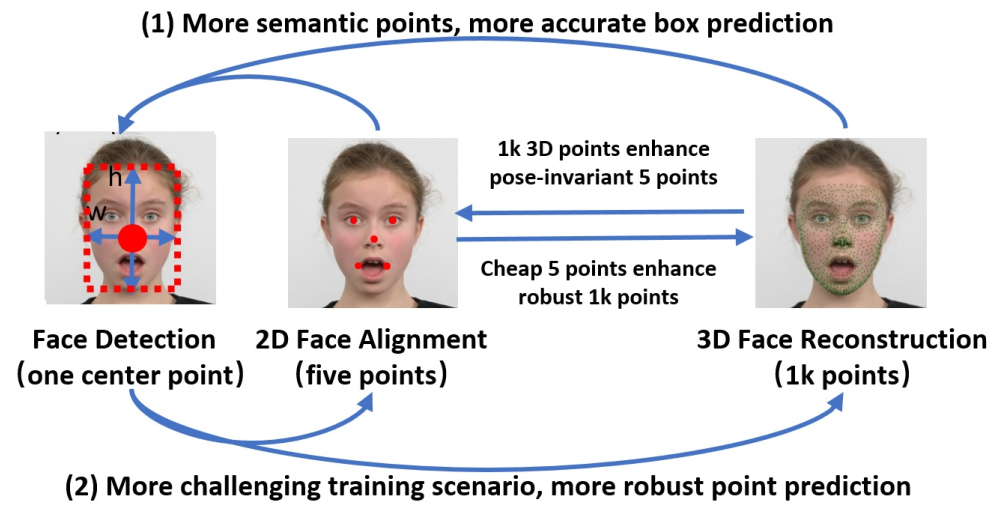
\includegraphics[scale=0.25]{LiteratureSurvey/RF_multiTaskBenefit}
        \label{fig:RF_multiTaskBenefit}
    }}
    \caption{Retina Face}
\end{figure}


%%%%%%%%%%
\section{Menpo 2D and 3D Benchmark}
The Menpo 2D and Menpo 3D benchmarks \citep{menpo} are datasets for multi-pose 2D and 3D facial landmark localization and tracking. In the Menpo 2D benchmark, different visible landmark configurations are designed for semi-frontal and profile faces, thus making the 2D face alignment full pose. In the Menpo 3D benchmark, a united landmark configuration is designed for both semi-frontal and profile faces based on the correspondence with a 3D face model, thus making face alignment not only full-pose but also corresponding to the real-world 3D space.

There are four different types of landmark configurations adopted in the dataset:
\begin{enumerate}
    \item Semi-frontal 2D landmarks: They correspond to the traditional facial landmarks as typically used in the literature. This configuration consists of 68 landmarks.
    \item Profile 2D landmarks: These are specially designed for profile faces where the traditional 2D landmarks are not suitable because a large number of landmarks are self-occluded. This configuration consists of 39 landmarks.
    \item 3DA-2D (3D Aware 2D) landmarks: They are defined as the 2D projections of the 3D landmarks on the image plane. This configuration consists of 84 landmarks.
    \item 3D landmarks: These are defined as the 3D coordinates of the facial landmarks; therefore, they bare information regarding the depth of the 3D face. This configuration consists of 84 landmarks.
\end{enumerate}

\begin{figure}[h]
    \centering
    \captionsetup[subfigure]{justification=centering}
    \subfloat[Semi-frontal 2D landmarks]{{
        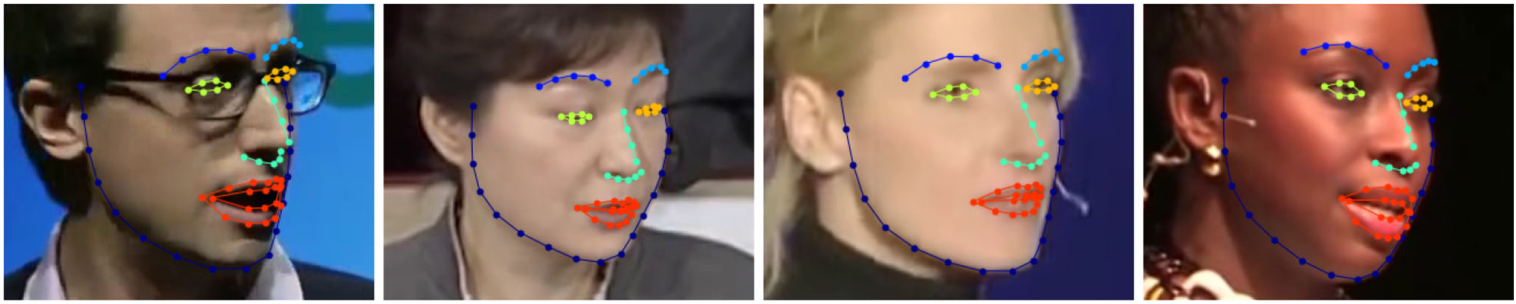
\includegraphics[scale=0.25]{LiteratureSurvey/Semi-frontal_2D}
        \label{fig:semi-frontal_2D}
        }}
    \quad
    \subfloat[3DA-2D landmarks]{{
        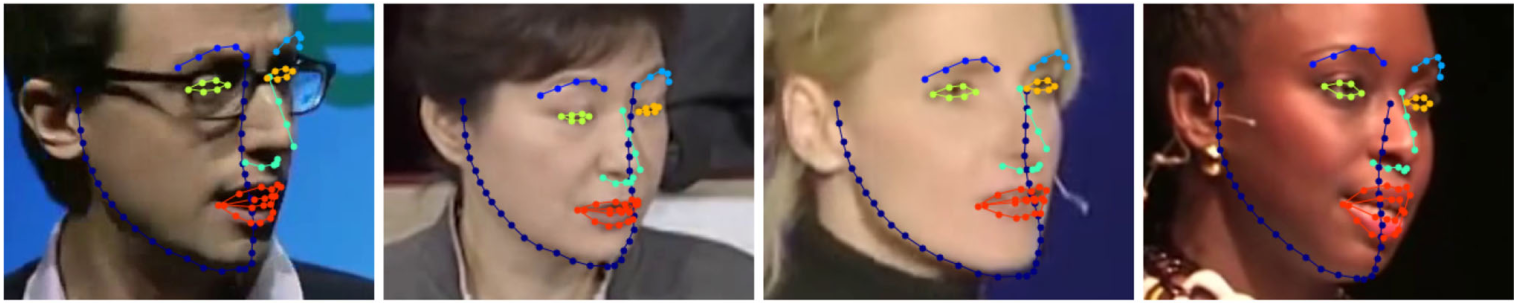
\includegraphics[scale=0.25]{LiteratureSurvey/3DA-2D}
        \label{fig:3DA-2D}
    }}
    \caption[Menpo: Semi-frontal 2D and 3DA-2D landmarks]{Menpo: Comparison of Semi-frontal 2D and 3DA-2D landmarks}
\end{figure}

\subsection{Ground-Truth creation of 3DA-2D and 3D Facial Landmarks}
Initially, a DCNN network \cite{dcnn} is employed to estimate the per frame 3DA-2D landmarks as a ground truth. Then, an energy minimization method is used to fit the combined identity and expression models on the landmarks of all frames of the video simultaneously. In more detail, a 3D Morphable Model is utilized as an identity and expression model. The vertices of these mesh models are rotated and translated using a linear view transformation to bring them into the camera reference frame:

\begin{equation}
\mathbf{v} = [v_x, v_y, v_z]^T = \mathbf{R}_v \mathbf{x} + \mathbf{t}_v
\end{equation}

where $\mathbf{R}_v$ and $\mathbf{t}_v$ are the camera's 3D rotation and translation components, respectively. Then, the camera projection is applied. For the sake of computational efficiency and stability, a scaled orthographic camera is considered, i.e., the 2D location of the 3D point $\mathbf{x}'$ is given by:

\begin{equation}
\mathbf{x}' = \sigma [v_x, v_y]^T
\end{equation}

where $\sigma$ is the scale parameter of the orthographic camera. Then, an optimization method using energy minimization is used to fit the obtained 2D coordinates to obtain the parameters of the model.


%%%%%%%%%%
\section{Comparison of Face Detectors}
The input face and eyes have to be extracted before they can be fed to the neural network. We explored several face detectors, as discussed in above sections, in order to figure out the best extractor. Precision-Recall curves and Average Precision (AP) scores are widely used as standard metrics to compare object detection algorithms (the face being the object in this work).

Precision measures the ability of a model to detect the true positives (i.e., faces) with high accuracy and low error. It is defined as the ratio of true positives to all the positive detections reported by the model. Recall is the ability of the model to detect all the the true positives present in the data. It is defined as the ratio of true positives to the sum of true positives and false negatives. The Precision-Recall curve is often plotted to negotiate a trade-off between the precision and recall values of a detection model. The area under the Precision-Recall curve quantifies this trade-off, which is called the Average Precision (AP) score of the model.

\begin{equation}
\begin{split}
Precision & = \frac{TP}{TP + FP} \\
Recall & = \frac{TP}{TP + FN}
\end{split}
\end{equation}
where,

\quad TP = True Positives

\quad FP = False Positives

\quad FN = False Negatives

Figure \ref{fig:result_allDetectors} compares the precision-recall curves of various detectors discussed in earlier chapter. From these results, it can be seen that DSFD works the best on our dataset, with the highest AP score at various IoU thresholds. Other detectors like Retina Face, S3FD, and LFFD are competitively accurate with DSFD, and at a reasonable IoU threshold of 0.5 or 0.6, the difference in AP scores is not very significant. But the YOLOv5 Face detector performs the worst among all. A reasonable explanation could be that all others are dedicated face detectors with dedicated pipelines for face detection, whereas YOLOv5 Face is just an extension of the YOLOv5 object detector.

\begin{figure}[h]
    \centering
    \captionsetup[subfigure]{justification=centering}
    \subfloat{{
        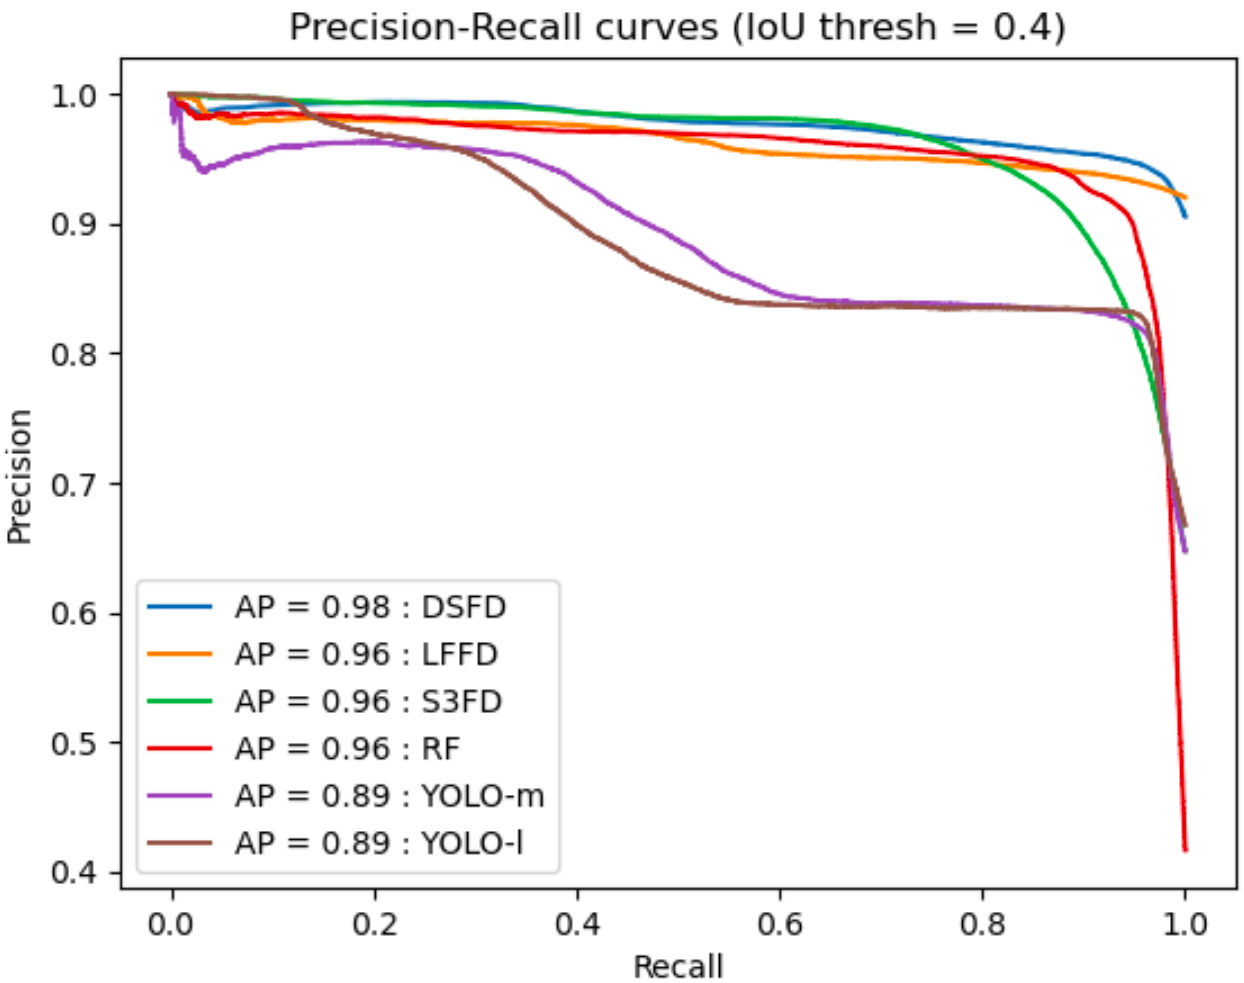
\includegraphics[width=0.45\textwidth]{LiteratureSurvey/DetectorAcc_Thresh-0.4}
        }}
    \quad
    \subfloat{{
        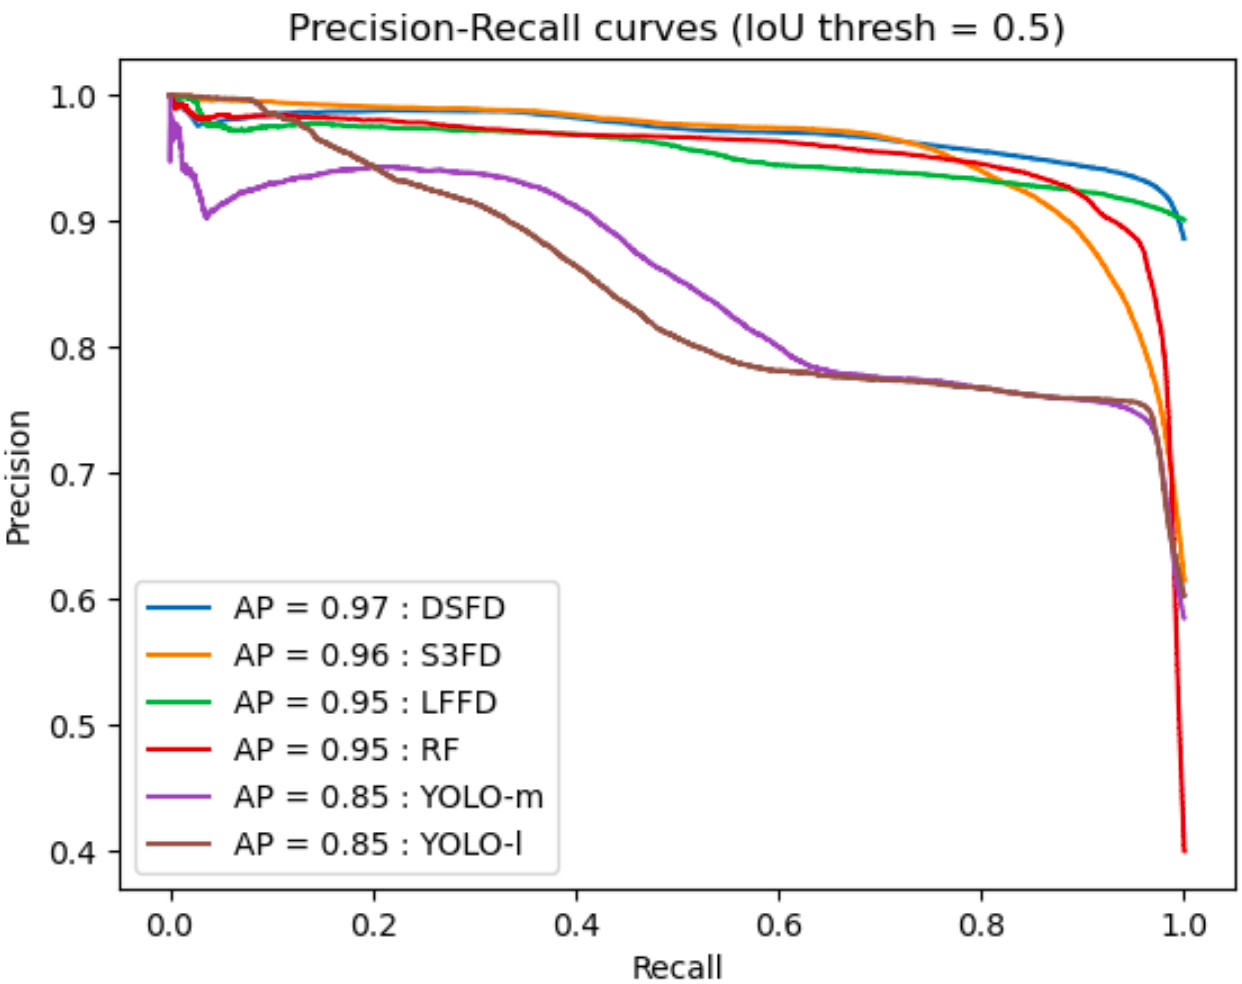
\includegraphics[width=0.45\textwidth]{LiteratureSurvey/DetectorAcc_Thresh-0.5}
    }}
    \quad
    \subfloat{{
        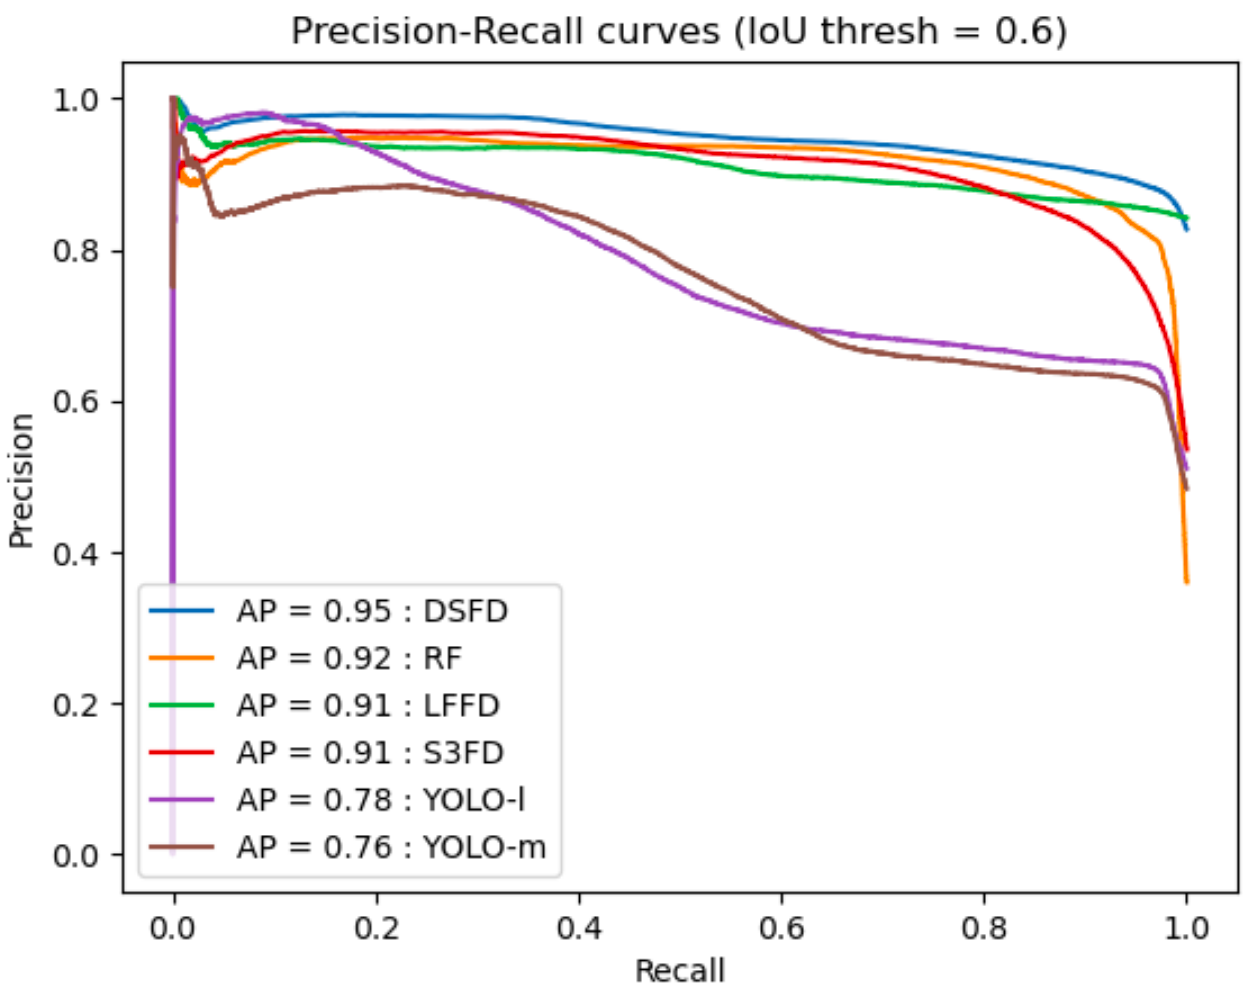
\includegraphics[width=0.45\textwidth]{LiteratureSurvey/DetectorAcc_Thresh-0.6}
    }}
    \quad
    \subfloat{{
        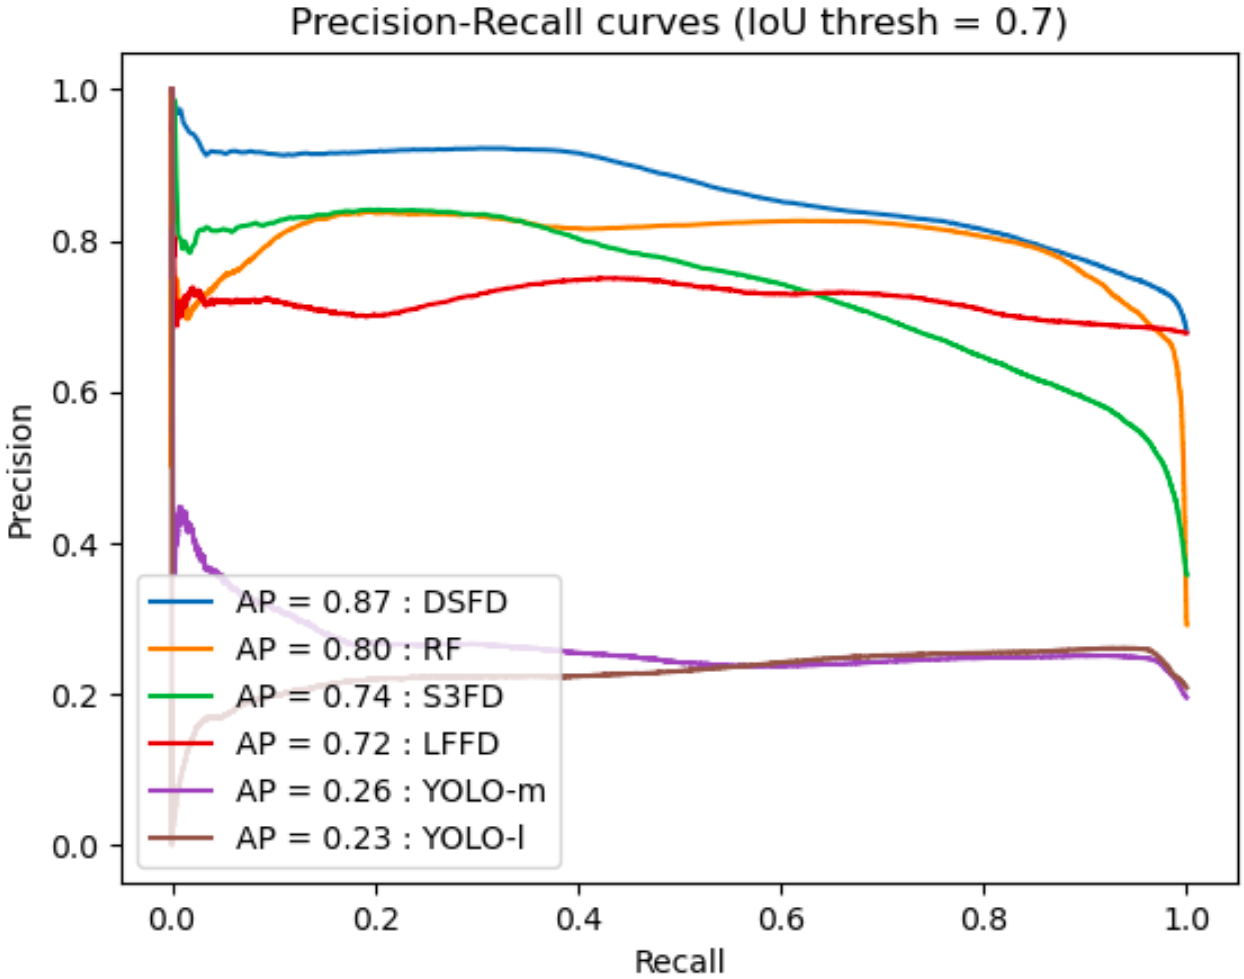
\includegraphics[width=0.45\textwidth]{LiteratureSurvey/DetectorAcc_Thresh-0.7}
    }}
    \caption{Accuracy comparison of various detectors}
    \label{fig:result_allDetectors}
\end{figure}

\begin{figure}[h]
  \centering
    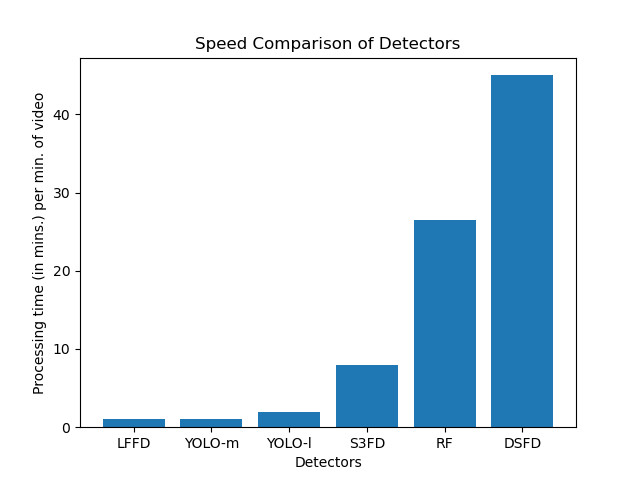
\includegraphics[scale=0.6]{LiteratureSurvey/Result_speed}
    \caption{Speed comparison of various detectors}
    \label{fig:result_speed}
\end{figure}

Out of all detectors used, the speed of DSFD is the slowest, as expected from the study of its architecture. It has a 2-stage pipeline, namely Original Feature Shot and Enhance Feature Shot which increases the runtime of DSFD. On the other hand, YOLOv5 Face and LFFD are the fastest detectors and can be used for real-time face detection applications. For an effective accuracy-speed trade-off, Retina Face is an excellent detector. So, for all extractions in our experiments, we used the Retina Face detector.
\chapter{Datasets}

We perform several experiments and ablation studies on some gaze tracking datasets in order to demonstrate the versatility of our method. There are three datasets used in this work which vary in terms of their nature (regression versus classification), ground truths (2-Way versus 3-Way), and the curation methodologies adopted (well-curated versus uncurated), which are discussed in the next sections.


%%%%%%%%%%
\section{3-Way UK Dataset}
This dataset is collected in the UK from an \href{https://drive.google.com/file/d/124HQbKAsR6YVIeK-IArFKTnjU8MRNNjh/view?usp=sharing}{Android app developed by Aditya Modi} from our team for the creation of the 3-Way gaze classification dataset. The app displays some objects in the left, middle and right regions of the screen, one at a time, as shown in figure \ref{fig:3wayUKdata}. The subject is asked to keep tracking the object as it appears on the screen in different regions while the front camera records the face of the subject.

\begin{figure}[h]
  \centering
    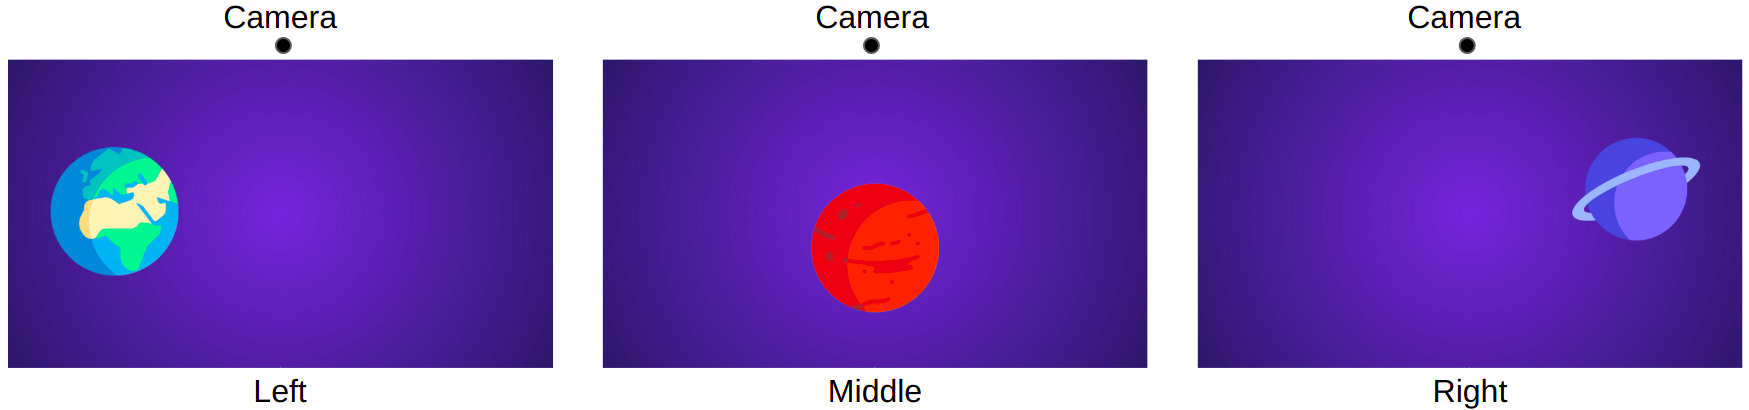
\includegraphics[width=0.8\textwidth]{Dataset/3-Way_UK_dataset}
    \caption{3-Way UK Dataset}
    \label{fig:3wayUKdata}
\end{figure}

\begin{figure}[h]
  \centering
    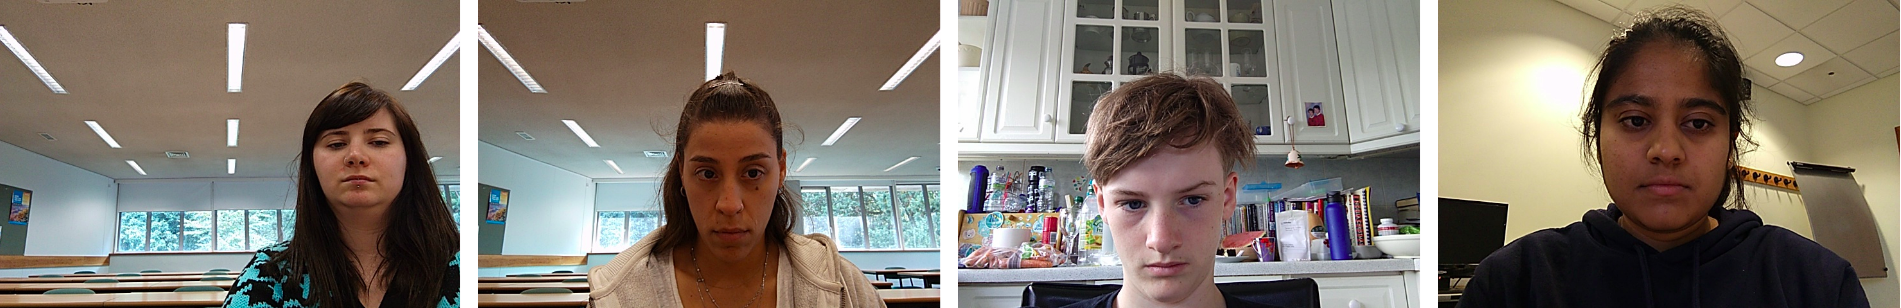
\includegraphics[width=1.0\textwidth]{Dataset/3Way_UK_subjects}
    \caption{Some examples from 3-Way UK Dataset}
    \label{fig:3wayUKdata_examples}
\end{figure}

It contains one of the three-class labels (Left, Middle, or Right) for each image frame. The device used for the collection of data is Huawei MediaPad M3 Lite 10 tablet (also referred to as \emph{UK device} here onwards). The camera in this device is located at the center of the long edge of the screen. The camera location is an important factor in the device specifications because the gaze of the subject (either XY coordinates or gaze classes) are defined w.r.t. the camera. In case of XY coordinate regression, the origin is defined at the camera location, and in the case of gaze classification, the divisions of the screen region are assigned taking into consideration the location of the camera.

The dataset contains 23 different subjects (samples shown in figure \ref{fig:3wayUKdata_examples}), each performing the task several times at different locations and in different lighting conditions, poses, etc. It contains a total of 539508 frames which are split into the train, val and test in a ratio of approximately 7:1:2 with 369835, 51998, and 117675 frames, respectively.


%%%%%%%%%%
\section{Filtered 2-Way UK Dataset}
Since we are also interested in 2-way along with 3-way gaze classification, we prepare a customized version of the 2-way gaze classification dataset from the 3-way UK dataset by simply removing the frames with "Middle" as the ground truth. Note that the resulting 2-way dataset has a buffer region in the middle where there are no frames in the dataset. So in that sense, it is a well-curated dataset.

The resulting dataset contains a total of 420811 frames which are split into the train, val and test in a ratio of approximately 7:1:2 with 288477, 40555, and 91779 frames, respectively.


%%%%%%%%%%
\section{2-Way Nottingham START Dataset}
The 2-way Nottingham START dataset is created by the Preferential Looking task being performed by children as a part of the START project in Nottingham. The app displays a social and a non-social video clip simultaneously on the screen; one displayed on the left and the other on the right side of the screen, randomly, as shown in figure \ref{fig:2waySTARTdata}. By recording the face and gazes of the children, this task gauges the social preference of the children.

% \begin{figure}[h]
%   \centering
%     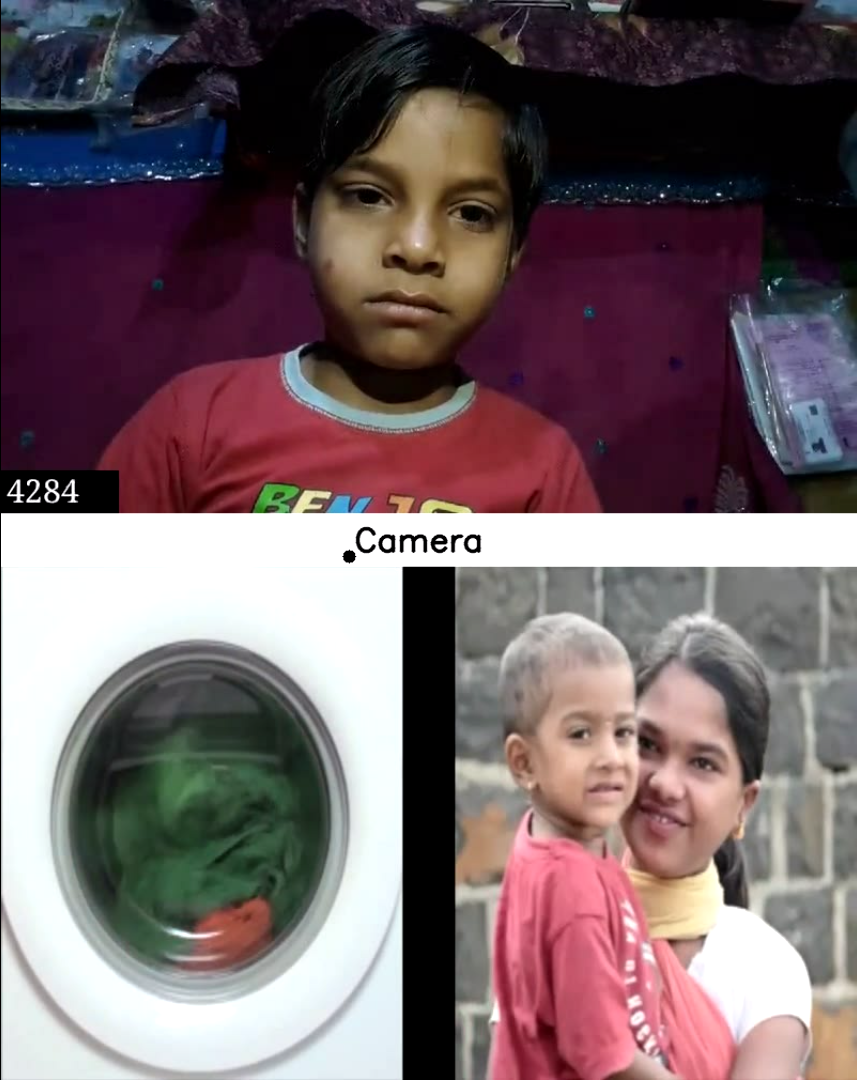
\includegraphics[width=0.38\textwidth]{Dataset/2-Way_START_dataset}
%     \caption{2-Way START Dataset}
%     \label{fig:2waySTARTdata}
% \end{figure}

\begin{figure}[h]
    \centering
    \captionsetup[subfigure]{justification=centering}
    \subfloat[Preferential Looking task]{{
        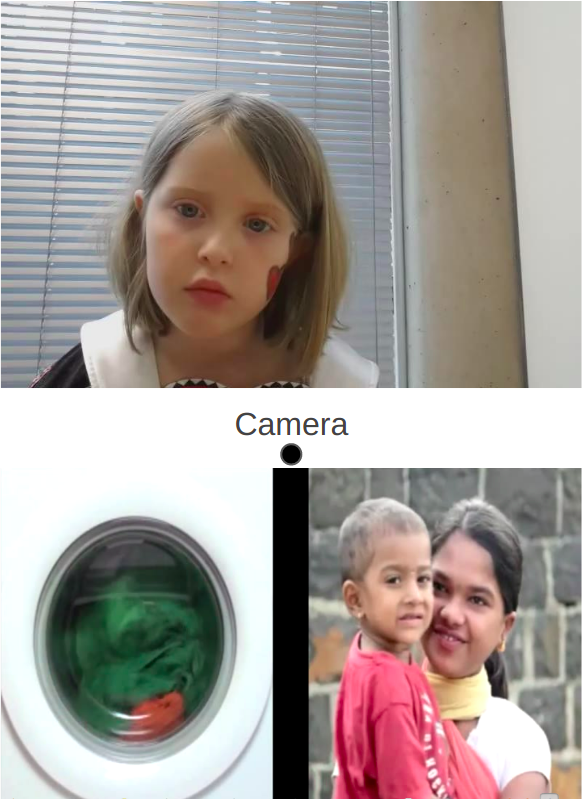
\includegraphics[width=0.3\textwidth,valign=m]{Dataset/2Way_Nottingham_START}
        }}
    \quad
    \subfloat[3rd person view of Preferential Looking task]{{
        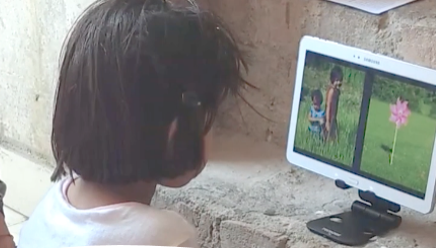
\includegraphics[scale=0.25,valign=m]{Dataset/3rdPersonView_PrefLooking}
    }}
    \caption{2-Way START Dataset collected using Preferential looking task}
    \label{fig:2waySTARTdata}
\end{figure}

It contains one of the two class labels (Left or Right) for each image frame. The device used for the collection of data is Samsung Note 10 SM P600 tablet (also referred to as \emph{START device} here onwards). The device dimensions are 24 cm x 17 cm and the camera in this device is located at an offset of 2 cm towards the left from the center of the long edge of the screen. Note that this dataset is not an in-the-wild dataset purely because although the START app was used for dataset collection, the videos were recorded in a lab environment.

The dataset contains 11 different subjects, each performing the Preferential Looking task. It contains a total of 7917 frames which are split into the train, val and test in a ratio of approximately 7:1:2 with 5541, 791, and 1585 frames, respectively.
\chapter{Proximity Preserving Face Redaction}

Face proximity preservation during redaction is crucial for gauging the attention of the subject. We are mainly interested in the relative back-and-forth motion of the face instead of the actual distance of the face from the camera. In the following sections, we describe a method to get the relative proximity of the face from the camera while redacting the face.


%%%%%%%%%%
\section{Proximity using PnP Algorithm}


%%%
\subsection{Methodology}
We employ the PnP (Perspective-n-Point) algorithm to calculate the face proximity from the camera. The algorithm takes 3-D coordinates in an arbitrary world coordinate system as input together with the corresponding 2-D image coordinates and the intrinsic camera parameters, and outputs the extrinsic camera parameters (translation and rotation), i.e., the pose and location of the camera w.r.t. the object defined in an object coordinate system.

We first calibrate the camera using a chessboard pattern and obtain the intrinsic parameters of the camera. Then, we calculate the 3-D facial landmarks (figure \ref{fig:retinaFace3Dlandmarks}) using the Retina Face landmark detector along with redacting the face. Retina Face outputs 68 3-D landmarks in pixel units with the coordinate system centered at the nose-tip. These 3-D coordinates form the 3-D coordinates input to the PnP algorithm. Since Retina Face predicts the 3-D facial landmarks in the pixel coordinate system, the XY of 3-D coordinates forms the corresponding 2-D image coordinates. By using the PnP algorithm, we obtain the proximity of the nose-tip from the camera in pixel units.

\begin{figure}[h]
    \centering
    \captionsetup[subfigure]{justification=centering}
    \subfloat{{
        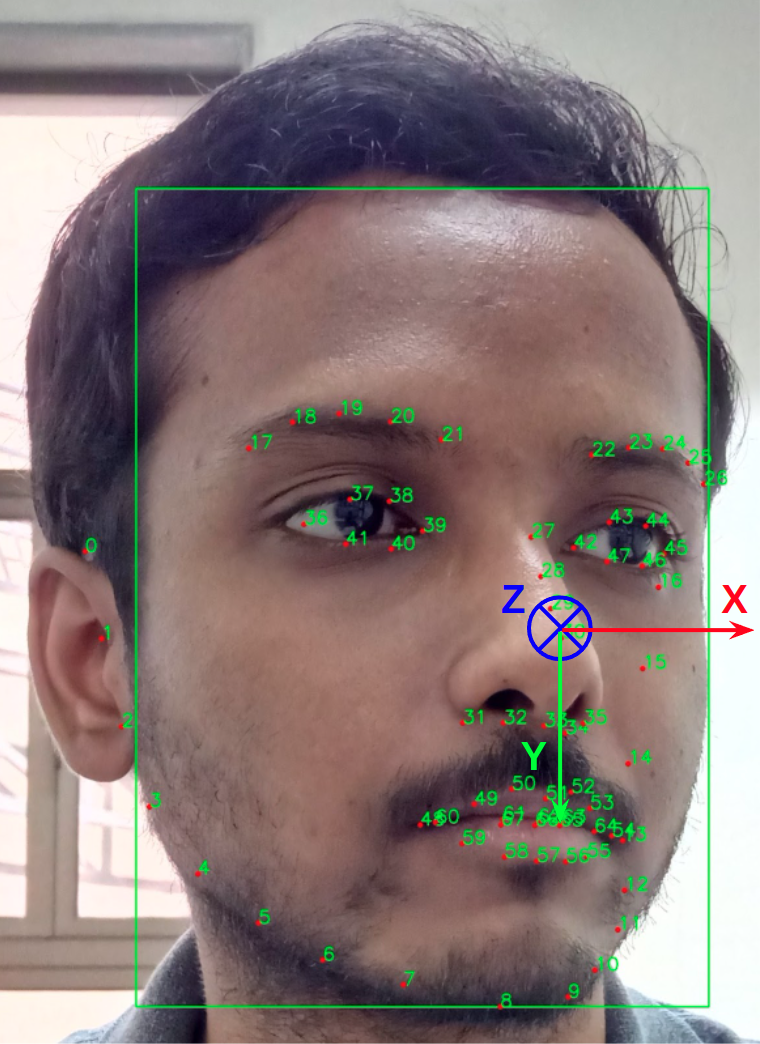
\includegraphics[scale=0.15,valign=m]{DistancePreservingRedaction/RetinaFaceCoordSystem}
        }}
    \quad
    \subfloat{{
        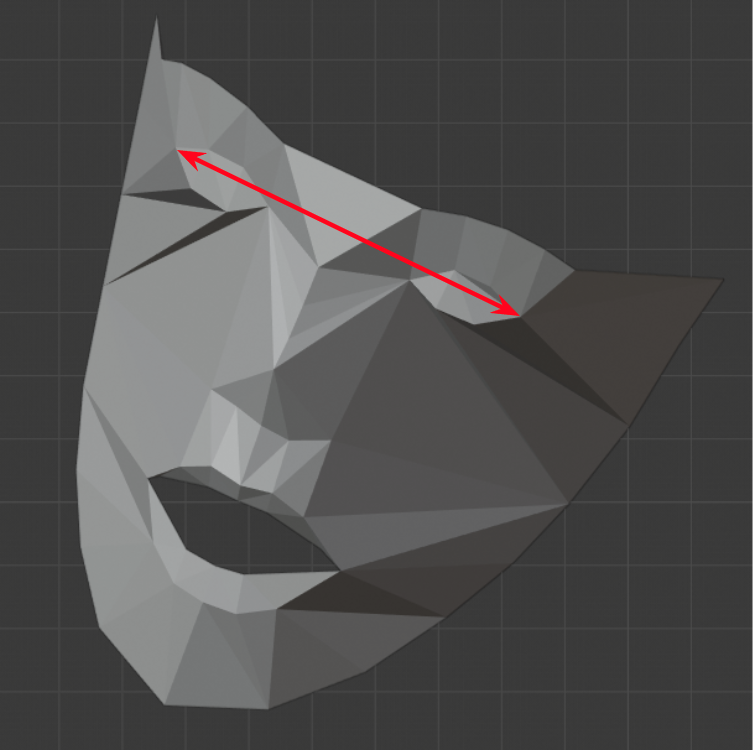
\includegraphics[scale=0.15,valign=m]{DistancePreservingRedaction/EyeExtremitiesDist}
    }}
    \caption{Retina Face: 3-D facial landmarks}
    \label{fig:retinaFace3Dlandmarks}
\end{figure}

Retina Face uses the same coordinate regression method used in Menpo \citep{menpo}, in which a deep neural network is trained jointly for regressing the 2-D and 3-D facial landmark coordinates. This uses a scaled orthographic camera model and scales the world coordinate system to the pixel coordinate system. Thus, the 3-D coordinates output by Retina Face need to be re-scaled back from pixel to world coordinate system. To achieve this, we map the euclidean pixel distance between the two extremes of the eyes (left-most corner of the left eye and right-most corner of the right eye) to the measurements taken in world units in cm. The scale conversion factor thus obtained is used to convert the distance from pixel to cm.


\subsection{Experiments}
To test the above method, we perform experiments in which we record the videos of some subjects gradually going away from the camera and subsequently coming closer to the camera. We then calculate the face proximity of each frame in the video and plot the proximity versus time curve.

\begin{figure}[h]
    \centering
    \captionsetup[subfigure]{justification=centering}
    \subfloat{{
        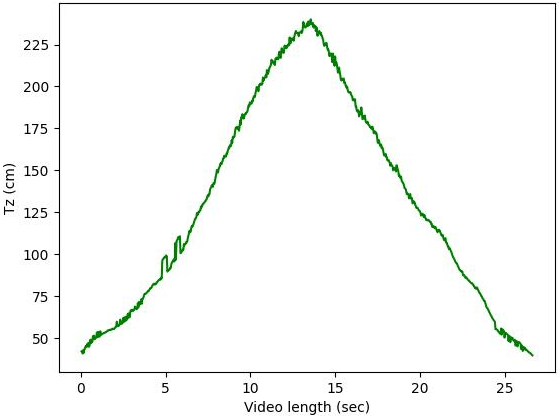
\includegraphics[scale=0.35]{DistancePreservingRedaction/plot-1}
        }}
    \quad
    \subfloat{{
        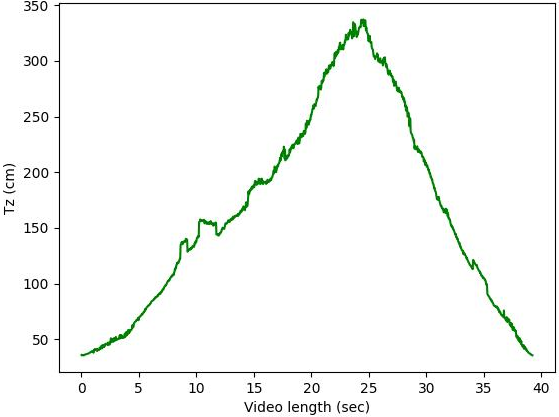
\includegraphics[scale=0.35]{DistancePreservingRedaction/plot-2}
    }}
    \quad
    \subfloat{{
        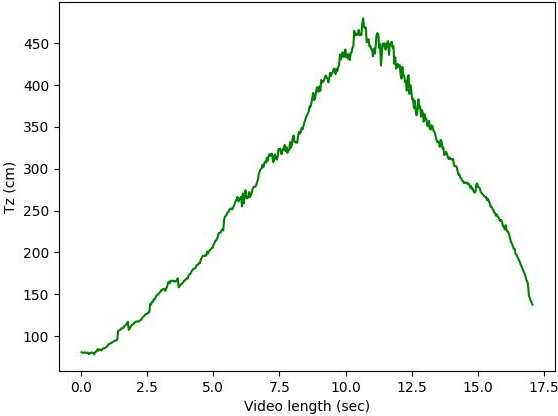
\includegraphics[scale=0.35]{DistancePreservingRedaction/plot-3}
    }}
    \quad
    \subfloat{{
        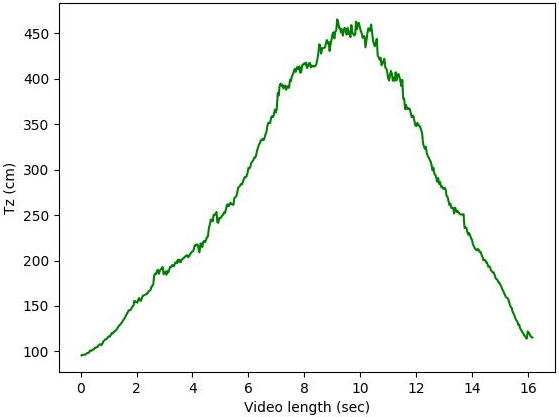
\includegraphics[scale=0.35]{DistancePreservingRedaction/plot-4}
    }}
    \caption[Proximity v/s Time curves]{Examples of Proximity v/s Time of video Curves}
    \label{fig:distCurve}
\end{figure}

\begin{figure}[h]
  \centering
    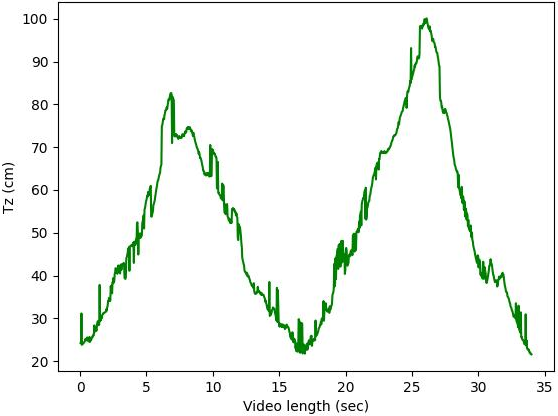
\includegraphics[scale=0.35]{DistancePreservingRedaction/plot-6}
    \caption[Proximity v/s Time curve in-the-wild]{Proximity v/s Time of video Curve for in-the-wild video}
    \label{fig:distCurve_inTheWild} 
\end{figure}

The curves in figure \ref{fig:distCurve} show some examples of facial proximity versus time plots we obtained for some of the videos. The videos on which we calculate these plots can be found \href{https://drive.google.com/drive/folders/1HEZISJiaaP0LAooNuELbls8TPWqtTL0M?usp=sharing}{here}.

We also simulated the in-the-wild nature of the 2-way START dataset where the subjects are relatively closer to the camera and the facial proximity fluctuates back and forth much more rapidly, along with large variations in the pose. In this video, the subject moves back and forth twice with large variations in pose, and as expected, there are two peaks in the proximity versus time curve shown in figure \ref{fig:distCurve_inTheWild}.

We also calculated the face proximity values for some images with measured ground truth values (the images along with their ground truths can be found \href{https://drive.google.com/drive/folders/1MsDul6SAmFN9JhgleApR6tdFm79J5AoK?usp=sharing}{here}). Table \ref{tab:proximityOnGrTrImages} shows the ground truth and the values predicted by our algorithm.

\begin{table}[h]
  \centering
    \caption{Face Proximity on Images with Ground Truths}
    \label{tab:proximityOnGrTrImages}
    \begin{tabular}{ | >{\centering\arraybackslash} m{2cm} || >{\centering\arraybackslash} m{1cm} | >{\centering\arraybackslash} m{1cm} | >{\centering\arraybackslash} m{1cm} | >{\centering\arraybackslash} m{1cm} | >{\centering\arraybackslash} m{1cm} | >{\centering\arraybackslash} m{1cm} | >{\centering\arraybackslash} m{1cm} |
    >{\centering\arraybackslash} m{1cm} |} 
        \hline
        \textbf{Ground Truth (cm)} & 54.3 & 71.5 & 101 & 126 & 177.6 & 224.1 & 271.1 & 321.5\\
        \hline
        \textbf{Prediction (cm)} & 65.9 & 85.7 & 121.7 & 149.9 & 211.6 & 261.1 & 320.1 & 381.1\\
        \hline
    \end{tabular}
\end{table}
\chapter{Proximity Preserving Face Redaction}

Face proximity preservation during redaction is crucial for gauging the attention of the subject. We are mainly interested in the relative back-and-forth motion of the face instead of the actual distance of the face from the camera. In the following sections, we describe a method to get the relative proximity of the face from the camera while redacting the face.


%%%%%%%%%%
\section{Proximity using PnP Algorithm}


%%%
\subsection{Methodology}
We employ the PnP (Perspective-n-Point) algorithm to calculate the face proximity from the camera. The algorithm takes 3-D coordinates in an arbitrary world coordinate system as input together with the corresponding 2-D image coordinates and the intrinsic camera parameters, and outputs the extrinsic camera parameters (translation and rotation), i.e., the pose and location of the camera w.r.t. the object defined in an object coordinate system.

We first calibrate the camera using a chessboard pattern and obtain the intrinsic parameters of the camera. Then, we calculate the 3-D facial landmarks (figure \ref{fig:retinaFace3Dlandmarks}) using the Retina Face landmark detector along with redacting the face. Retina Face outputs 68 3-D landmarks in pixel units with the coordinate system centered at the nose-tip. These 3-D coordinates form the 3-D coordinates input to the PnP algorithm. Since Retina Face predicts the 3-D facial landmarks in the pixel coordinate system, the XY of 3-D coordinates forms the corresponding 2-D image coordinates. By using the PnP algorithm, we obtain the proximity of the nose-tip from the camera in pixel units.

\begin{figure}[h]
    \centering
    \captionsetup[subfigure]{justification=centering}
    \subfloat{{
        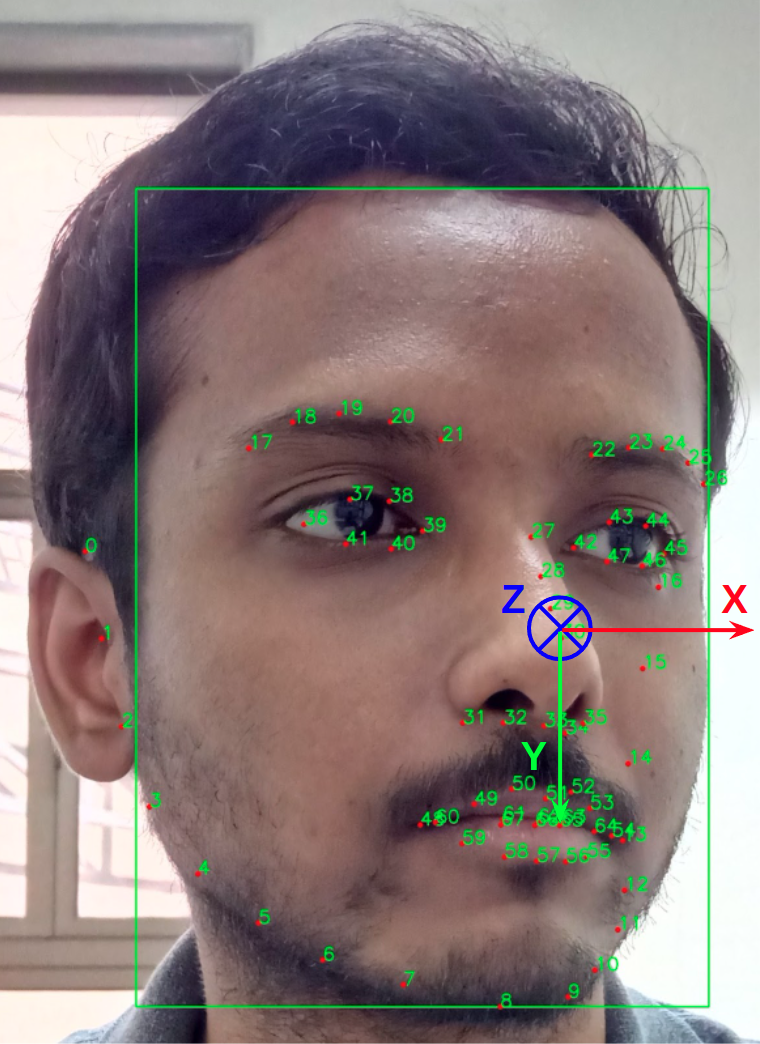
\includegraphics[scale=0.15,valign=m]{DistancePreservingRedaction/RetinaFaceCoordSystem}
        }}
    \quad
    \subfloat{{
        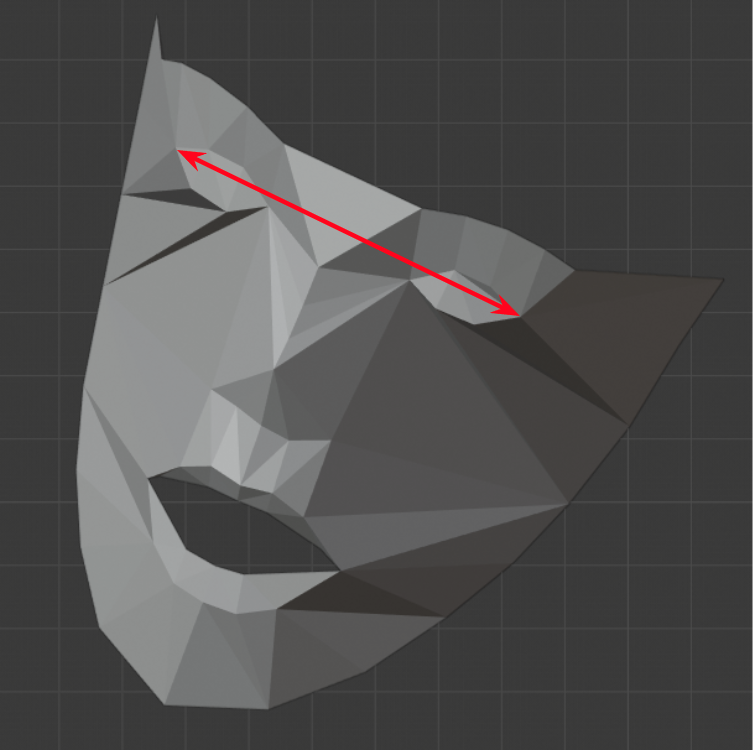
\includegraphics[scale=0.15,valign=m]{DistancePreservingRedaction/EyeExtremitiesDist}
    }}
    \caption{Retina Face: 3-D facial landmarks}
    \label{fig:retinaFace3Dlandmarks}
\end{figure}

Retina Face uses the same coordinate regression method used in Menpo \citep{menpo}, in which a deep neural network is trained jointly for regressing the 2-D and 3-D facial landmark coordinates. This uses a scaled orthographic camera model and scales the world coordinate system to the pixel coordinate system. Thus, the 3-D coordinates output by Retina Face need to be re-scaled back from pixel to world coordinate system. To achieve this, we map the euclidean pixel distance between the two extremes of the eyes (left-most corner of the left eye and right-most corner of the right eye) to the measurements taken in world units in cm. The scale conversion factor thus obtained is used to convert the distance from pixel to cm.


\subsection{Experiments}
To test the above method, we perform experiments in which we record the videos of some subjects gradually going away from the camera and subsequently coming closer to the camera. We then calculate the face proximity of each frame in the video and plot the proximity versus time curve.

\begin{figure}[h]
    \centering
    \captionsetup[subfigure]{justification=centering}
    \subfloat{{
        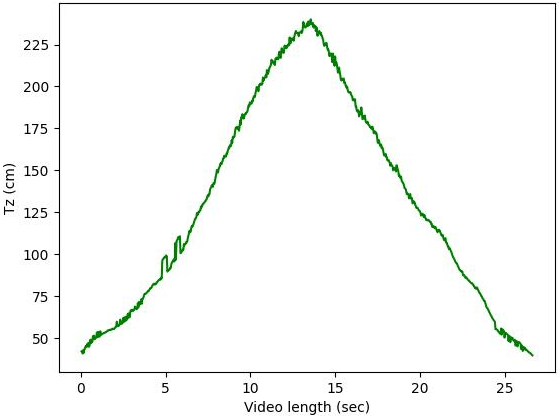
\includegraphics[scale=0.35]{DistancePreservingRedaction/plot-1}
        }}
    \quad
    \subfloat{{
        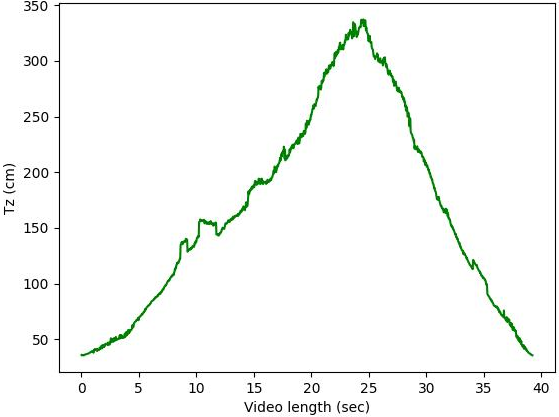
\includegraphics[scale=0.35]{DistancePreservingRedaction/plot-2}
    }}
    \quad
    \subfloat{{
        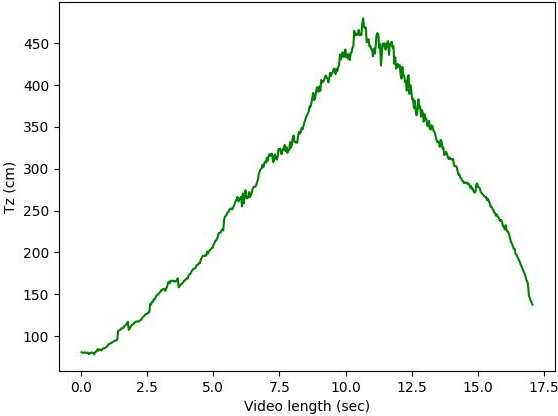
\includegraphics[scale=0.35]{DistancePreservingRedaction/plot-3}
    }}
    \quad
    \subfloat{{
        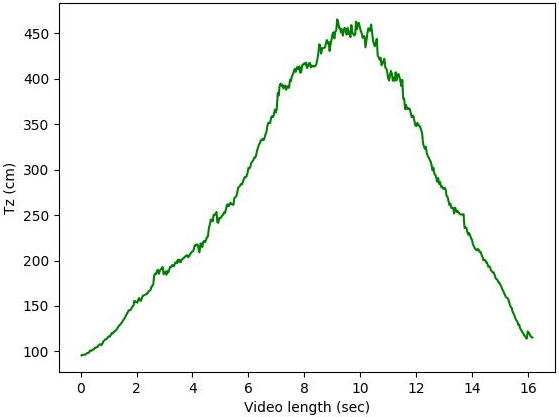
\includegraphics[scale=0.35]{DistancePreservingRedaction/plot-4}
    }}
    \caption[Proximity v/s Time curves]{Examples of Proximity v/s Time of video Curves}
    \label{fig:distCurve}
\end{figure}

\begin{figure}[h]
  \centering
    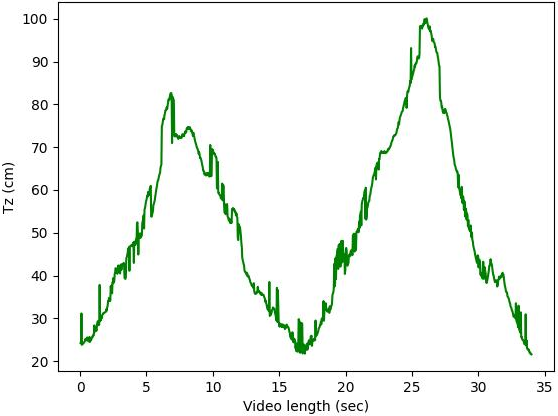
\includegraphics[scale=0.35]{DistancePreservingRedaction/plot-6}
    \caption[Proximity v/s Time curve in-the-wild]{Proximity v/s Time of video Curve for in-the-wild video}
    \label{fig:distCurve_inTheWild} 
\end{figure}

The curves in figure \ref{fig:distCurve} show some examples of facial proximity versus time plots we obtained for some of the videos. The videos on which we calculate these plots can be found \href{https://drive.google.com/drive/folders/1HEZISJiaaP0LAooNuELbls8TPWqtTL0M?usp=sharing}{here}.

We also simulated the in-the-wild nature of the 2-way START dataset where the subjects are relatively closer to the camera and the facial proximity fluctuates back and forth much more rapidly, along with large variations in the pose. In this video, the subject moves back and forth twice with large variations in pose, and as expected, there are two peaks in the proximity versus time curve shown in figure \ref{fig:distCurve_inTheWild}.

We also calculated the face proximity values for some images with measured ground truth values (the images along with their ground truths can be found \href{https://drive.google.com/drive/folders/1MsDul6SAmFN9JhgleApR6tdFm79J5AoK?usp=sharing}{here}). Table \ref{tab:proximityOnGrTrImages} shows the ground truth and the values predicted by our algorithm.

\begin{table}[h]
  \centering
    \caption{Face Proximity on Images with Ground Truths}
    \label{tab:proximityOnGrTrImages}
    \begin{tabular}{ | >{\centering\arraybackslash} m{2cm} || >{\centering\arraybackslash} m{1cm} | >{\centering\arraybackslash} m{1cm} | >{\centering\arraybackslash} m{1cm} | >{\centering\arraybackslash} m{1cm} | >{\centering\arraybackslash} m{1cm} | >{\centering\arraybackslash} m{1cm} | >{\centering\arraybackslash} m{1cm} |
    >{\centering\arraybackslash} m{1cm} |} 
        \hline
        \textbf{Ground Truth (cm)} & 54.3 & 71.5 & 101 & 126 & 177.6 & 224.1 & 271.1 & 321.5\\
        \hline
        \textbf{Prediction (cm)} & 65.9 & 85.7 & 121.7 & 149.9 & 211.6 & 261.1 & 320.1 & 381.1\\
        \hline
    \end{tabular}
\end{table}
\chapter{Results and Discussions}

\section{Conclusions}
Redaction is an important procedure in order to preserve privacy and has applications in many domains like dataset preparation, remote exam settings, etc. In this work, we presented the feature preserving approach to face redaction, which is very crucial to undertake before the essential features are lost during redaction. We demonstrated the feature-preserving nature of our approaches on 3-way and 2-way gaze classification and facial proximity preservation via several experiments and ablation studies. \\

The post-classification approach is the most straightforward way for gaze classification in the presence of an already trained regression model. These models do not generalize well across datasets due to domain shift in data distribution. In order to learn a robust model, the model needs to be trained (i.e., tuned) on the target dataset, which enables it to adapt to the data distribution shift between the source and target dataset. The tuning process can be done on very small data and still train the model for state-of-the-art accuracy values. \\

We demonstrated via various redaction schemes (blurred or blacked out face or eyes) the robustness of our feature-preserving face redaction. The results show that gaze classification on redacted images is as accurate as that performed on un-redacted images. The ablation studies with redaction of eyes demonstrated the importance of eyes for gaze classification and emphasized on the fact that the model is able to learn from the eye crops. We also explored the explicit need for training a model on redacted faces, and via elaborate experiments, we concluded that tuning the model with visible faces works equally well for gaze prediction on redacted faces. \\

The direct classification approach, where a classifier is trained from scratch, showed that to learn robust features, a significant amount of data is required for training. Also, the results of the classifier model trained on UK data and tested on START data demonstrated that, unlike the regression model, the classification model generalizes well across datasets and is able to overcome the domain shift in data distribution arising due to the differences in the source and target datasets.

Finally, we utilized a 2-way gaze classification model for the task of 3-way gaze classification without requiring any training and still obtaining high accuracy. This demonstrates the robustness of our 2-way classifier and the ability of the model to predict the left and right gaze with high confidence. We also preserved the relative face proximity feature by using the facial landmarks and demonstrated the expected trend of proximity versus the time of the video to be matching our results.

We also calculated facial proximity values by using the facial landmarks output by Retina Face and employing the PnP algorithm. We demonstrated the trend of proximity values on videos as well as on the images with measured ground truths. Another approach to facial proximity calculation is discussed in the Appendix.


\section{Future Scope}
We mentioned in section 4.3.1 that the post-classification approach suffers from device dependencies issues. We established this by training a regression model on MIT data and testing for classification on filtered 2-way UK data. In order to further strengthen the proof, one could also establish the device dependency by training a regression model on filtered 2-way UK data and testing for classification on MIT data. Note that in order to achieve this, one would first need to extract the ground-truth stimulus coordinates displayed on the 3-way gaze application.\\

We have demonstrated the robustness of our methods via several model tuning experiments mentioned in the previous chapters. Another approach to gaze preserving face redaction could be to build a neural network architecture that just takes the 3-D facial landmark features and the face grid as inputs and attempts to predict the gaze classes. Specifically, one could train and test the gaze classification task with only landmarks and a face grid supplied as input features (i.e., no face and eyes). This would result in a significant reduction in computation cost as the convolution layers would then not be required in the network architecture.

%****************************************************************
%                         Appendices                           
%****************************************************************
%% Additional, supporting material, such as codes, derivations, etc., can be placed in the appendix
\appendix
\chapter{Facial Proximity calculation: Orthographic to Perspective Method}
Retina Face uses the same coordinate regression method used in Menpo \citep{menpo}, which uses a scaled orthographic camera model and scales the world coordinate system to the pixel coordinate system. But the camera used to capture images in the real world actually follows a perspective camera model instead. Therefore, a possible approach to facial proximity calculation could be to try to first invert the scaled orthographic projection applied intrinsically by Retina Face, and then apply a perspective camera model to obtain the proximity.

In order to do so, we first formulate the landmark coordinate model of Retina Face as follows:

\begin{equation}
\label{eq:retinaFaceModel}
X_{RF} = O_{fst} ~\sigma ~T ~R ~X_W
\end{equation}

where, 

\qquad $X_{RF}$ = homogeneous 3-D landmark coordinates predicted by RetinaFace (4x1 matrix)

\qquad $O_{fst}$ = camera offset in pixel coordinates (4x4 matrix)

\qquad $\sigma$ = uniform scale parameter of scaled orthographic camera model (4x4 matrix)

\qquad $T$ = translation component of extrinsic camera parameters (4x4 matrix)

\qquad $R$ = rotation component of extrinsic camera parameters (4x4 matrix)

\qquad $X_W$ = homogeneous world coordinates of landmarks (4x1 matrix)

Then, we invert the orthographic projection as follows and apply the perspective camera model:

\begin{equation}
\label{eq:ortho2perspective}
s [x_{RF},~y_{RF},~1]^T = M_I ~[I | 0] ~T_z ~\sigma^{-1} ~O_{fst}^{-1} ~X_{RF}
\end{equation}

where,

\qquad $s$ = the homogeneous coordinate

\qquad $x_{RF}$, $y_{RF}$ = XY coordinates in the image

\qquad $M_I$ = intrinsic parameters of calibrated camera

\qquad $T_z$ = required proximity of face from camera\\

The above formulations explain an interesting mathematical approach to calculating the facial proximity. The idea is based on a set of transformations used to arrive at a perspective projection from an orthographic projection.


%******************************************************************
%                         Bibliography or References          
%******************************************************************  
\bibliography{mylit}     

%*******************************************************************
%                         List of publications               
%******************************************************************
% %%%
\listofpublications


\noindent Put your publications from the thesis here. The packages \texttt{multibib} or \texttt{bibtopic} or \texttt{biblatex} or enumerate environment or thebibliography environment etc. can be used to handle multiple different bibliographies in the document.








%%======================================================================
%%% Local Variables: 
%%% mode: latex
%%% TeX-master: "../mainrep"
%%% End: 







            

%*******************************************************************
%                        Acknowledgements                    
%******************************************************************* 
%%%
\acknowledgments

I would like to thank my supervisor, Prof. Sharat Chandran, for his constant encouragement and guidance. I would also like to thank my mentor Mr. Rahul Bishain for always helping me come up with new ideas and approaches to solve a problem. I would like to thank all my seniors, with a special mention of Aditya Modi, who developed the 3-Way app on which the 3-Wau dataset was collected. I would like to express my thanks to all members of ViGIL lab, my batch-mates and friends for their support throughout this journey.

\signature{\today}
%\signature[Indian Institute of Technology Bombay]{\today}

%========================================================================

%%% Local Variables: 
%%% mode: latex
%%% TeX-master: "../mainrep"
%%% End:            

%*******************************************************************
%                        About author                    
%*******************************************************************
% \colophon % remove this command while using this file.

% GAME OVER
%*******************************************************************
\end{document}

%%% Local Variables: 
%%% mode: latex
%%% TeX-master: t
%%% End: 
